\documentclass[9pt,a4paper,]{extarticle}

\usepackage{f1000_styles}

\usepackage[pdfborder={0 0 0}]{hyperref}

\usepackage[numbers]{natbib}
\bibliographystyle{unsrtnat}


%% maxwidth is the original width if it is less than linewidth
%% otherwise use linewidth (to make sure the graphics do not exceed the margin)
\makeatletter
\def\maxwidth{ %
  \ifdim\Gin@nat@width>\linewidth
    \linewidth
  \else
    \Gin@nat@width
  \fi
}
\makeatother

\usepackage{color}
\usepackage{fancyvrb}
\newcommand{\VerbBar}{|}
\newcommand{\VERB}{\Verb[commandchars=\\\{\}]}
\DefineVerbatimEnvironment{Highlighting}{Verbatim}{commandchars=\\\{\}}
% Add ',fontsize=\small' for more characters per line
\usepackage{framed}
\definecolor{shadecolor}{RGB}{248,248,248}
\newenvironment{Shaded}{\begin{snugshade}}{\end{snugshade}}
\newcommand{\AlertTok}[1]{\textcolor[rgb]{0.94,0.16,0.16}{#1}}
\newcommand{\AnnotationTok}[1]{\textcolor[rgb]{0.56,0.35,0.01}{\textbf{\textit{#1}}}}
\newcommand{\AttributeTok}[1]{\textcolor[rgb]{0.77,0.63,0.00}{#1}}
\newcommand{\BaseNTok}[1]{\textcolor[rgb]{0.00,0.00,0.81}{#1}}
\newcommand{\BuiltInTok}[1]{#1}
\newcommand{\CharTok}[1]{\textcolor[rgb]{0.31,0.60,0.02}{#1}}
\newcommand{\CommentTok}[1]{\textcolor[rgb]{0.56,0.35,0.01}{\textit{#1}}}
\newcommand{\CommentVarTok}[1]{\textcolor[rgb]{0.56,0.35,0.01}{\textbf{\textit{#1}}}}
\newcommand{\ConstantTok}[1]{\textcolor[rgb]{0.00,0.00,0.00}{#1}}
\newcommand{\ControlFlowTok}[1]{\textcolor[rgb]{0.13,0.29,0.53}{\textbf{#1}}}
\newcommand{\DataTypeTok}[1]{\textcolor[rgb]{0.13,0.29,0.53}{#1}}
\newcommand{\DecValTok}[1]{\textcolor[rgb]{0.00,0.00,0.81}{#1}}
\newcommand{\DocumentationTok}[1]{\textcolor[rgb]{0.56,0.35,0.01}{\textbf{\textit{#1}}}}
\newcommand{\ErrorTok}[1]{\textcolor[rgb]{0.64,0.00,0.00}{\textbf{#1}}}
\newcommand{\ExtensionTok}[1]{#1}
\newcommand{\FloatTok}[1]{\textcolor[rgb]{0.00,0.00,0.81}{#1}}
\newcommand{\FunctionTok}[1]{\textcolor[rgb]{0.00,0.00,0.00}{#1}}
\newcommand{\ImportTok}[1]{#1}
\newcommand{\InformationTok}[1]{\textcolor[rgb]{0.56,0.35,0.01}{\textbf{\textit{#1}}}}
\newcommand{\KeywordTok}[1]{\textcolor[rgb]{0.13,0.29,0.53}{\textbf{#1}}}
\newcommand{\NormalTok}[1]{#1}
\newcommand{\OperatorTok}[1]{\textcolor[rgb]{0.81,0.36,0.00}{\textbf{#1}}}
\newcommand{\OtherTok}[1]{\textcolor[rgb]{0.56,0.35,0.01}{#1}}
\newcommand{\PreprocessorTok}[1]{\textcolor[rgb]{0.56,0.35,0.01}{\textit{#1}}}
\newcommand{\RegionMarkerTok}[1]{#1}
\newcommand{\SpecialCharTok}[1]{\textcolor[rgb]{0.00,0.00,0.00}{#1}}
\newcommand{\SpecialStringTok}[1]{\textcolor[rgb]{0.31,0.60,0.02}{#1}}
\newcommand{\StringTok}[1]{\textcolor[rgb]{0.31,0.60,0.02}{#1}}
\newcommand{\VariableTok}[1]{\textcolor[rgb]{0.00,0.00,0.00}{#1}}
\newcommand{\VerbatimStringTok}[1]{\textcolor[rgb]{0.31,0.60,0.02}{#1}}
\newcommand{\WarningTok}[1]{\textcolor[rgb]{0.56,0.35,0.01}{\textbf{\textit{#1}}}}

% disable code chunks background
%\renewenvironment{Shaded}{}{}

% disable section numbers
\setcounter{secnumdepth}{0}

%% added by MLS, this is not in the F1000 style by default %%

\hypersetup{unicode=true,
            pdftitle={sSNAPPY: a R/Bioconductor package for single-sample directional pathway perturbation analysis},
            pdfkeywords={RNA-seq, pathway enrichment, R package, topology, KEGG, scRNA-seq},
            pdfborder={0 0 0},
            breaklinks=true}

%% End added by MLS %%

\setlength{\parindent}{0pt}
\setlength{\parskip}{6pt plus 2pt minus 1pt}


\usepackage{endfloat}
\usepackage{booktabs}
\usepackage{longtable}
\usepackage{booktabs}
\usepackage{longtable}
\usepackage{array}
\usepackage{multirow}
\usepackage{wrapfig}
\usepackage{float}
\usepackage{colortbl}
\usepackage{pdflscape}
\usepackage{tabu}
\usepackage{threeparttable}
\usepackage{threeparttablex}
\usepackage[normalem]{ulem}
\usepackage{makecell}
\usepackage{xcolor}

\begin{document}
\pagestyle{front}

\title{sSNAPPY: a R/Bioconductor package for single-sample directional pathway perturbation analysis}

\author[1]{Wenjun Liu\thanks{\ttfamily Corresponding Author wenjun.liu@adelaide.edu.au}}
\author[2,3,4,5]{Ville-Petteri Mäkinen}
\author[1]{Wayne D. Tilley}
\author[1,6,7]{Stephen M. Pederson}
\affil[1]{Dame Roma Mitchell Cancer Research Laboratories, Adelaide Medical School, Faculty of Health and Medical Sciences, University of Adelaide, Adelaide, Australia}
\affil[2]{Australian Centre for Precision Health, Cancer Research Institute, University of South Australia, Adelaide, Australia}
\affil[3]{Computational and Systems Biology Program, Precision Medicine Theme, South Australian Health and Medical Research Institute, Adelaide, Australia}
\affil[4]{Computational Medicine, Faculty of Medicine, University of Oulu, Oulu, Finland}
\affil[5]{Center for Life Course Health Research, Faculty of Medicine, University of Oulu, Oulu, Finland}
\affil[6]{Black Ochre Data Laboratories, Telethon Kids Institute, Adelaide, Australia}
\affil[7]{John Curtin School of Medical Research, Australian National University, Canberra, Australia}

\maketitle
\thispagestyle{front}

\begin{abstract}
When analysing RNA-Seq data, a common outcome is to detect biological pathways with significantly altered activity between the conditions under investigation. The most common strategies test for over-representation within pre-defined gene-sets for genes showing changed expression\citep{Subramanian2005-lx, Young2010-jw}, but without accounting for gene-gene interactions encoded by pathway topologies, and not being able to directly predict the directional change of pathway activity. To address these issues, we have deloped a single-sample pathway perturbation analysis method \href{https://bioconductor.org/packages/sSNAPPY}{\emph{sSNAPPY}}, now available as an R/Bioconductor package, which leverages pathway topology information to compute pathway perturbation scores, and predicts the potential direction of change across a set of pathways. Here, we demonstrate the use of \emph{sSNAPPY} by applying the method to public scRNA-seq data, derived from ovarian cancer patient tissues collected before and after chemotherapy. Not only were we able to replicate results reported in the original study, but \emph{sSNAPPY} was also able to detect significant perturbation of other biological processes, yielding far greater insight into the response to treatment. \emph{sSNAPPY} represents a novel pathway analysis strategy that takes into consideration of pathway topology to predict impacted biology pathways, both within related samples and across treatment groups. In addition to not relying on the detection of differentially expressed genes, the method and associated R package offer important flexibility and provide powerful visualisation tools.
\end{abstract}

\section*{Keywords}
RNA-seq, pathway enrichment, R package, topology, KEGG, scRNA-seq


\clearpage
\pagestyle{main}

\textbf{R version}: R version 4.2.3 (2023-03-15)

\textbf{Bioconductor version}: 3.16

\hypertarget{introduction}{%
\section{Introduction}\label{introduction}}

Using pathway enrichment analysis to gain biological insights from gene expression data is a pivotal step in the analysis and interpretation of RNA-seq data, for which numerous methods have been developed (reviewed in \citep{Maleki2020-ur, Mubeen2022-eq}).
Many existing methods tend to view pathways simply as a collection of gene names, as seen in those relying on the detection of differentially expressed genes and applying over-representation analysis (ORA) strategies, and those scoring all genes using functional class scoring (FCS), such as in Gene Set Enrichment Analysis (GSEA) \citep{Subramanian2005-lx}, arguably the most widely-used approach.
However, databases such as the Kyoto Encyclopaedia of Genes and Genomes (KEGG)\citep{OgataKEGGKyotoEncyclopediaa} and WikiPathways\citep{Martens2021} capture not only which genes are implicated in a certain biological process but also their interactions, activating or inhibitory roles, and their relative importance within the pathway, all of which are overlooked in ORA- and FCS-based approaches.

To fully utilise that additional information, the latest generation of pathway analysis approaches include many which are topology-based such as SPIA\citep{Tarca2009-nf}, DEGraph\citep{Jacob2012}, NetGSA\citep{Ma2016} and PRS\citep{Ibrahim2012}, as well as others which explicitly model inter-gene correlations\citep{Wu2012}.
Despite differences in the null hypotheses tested across these approaches, overall, they have demonstrated enhanced sensitivity and specificity due to their abilities to take gene-gene interconnections into account\citep{Nguyen2019-va, Ma2019}.
Nevertheless, most topology-based methods focus only on comparing activities of pathways between two treatment groups and cannot be used to score individual samples.
However, in heterogenous data where more than one factor may be influencing our observations\citep{Hanzelmann2013}, incorporating scoring within paired samples may be desirable and may be able to reveal more nuanced insights.
To address this gap, we present a Single-Sample Network and Pathway Perturbation analysis methodology called \href{https://bioconductor.org/packages/sSNAPPY}{\emph{sSNAPPY}}, available as an R/Bioconductor package.
This article defines how \emph{sSNAPPY} computes changes in gene expression within paired samples, and propagates this through gene-set topologies to predict the perturbation in pathway activities within paired samples, before providing summarised results across an entire dataset which would include more robust levels of biological replication.
The practical usage of the \emph{sSNAPPY} R/Bioconductor package will be illustrated through the analysis of a public scRNA-seq dataset using pseudo-bulk strategies.

\hypertarget{methods}{%
\section{Methods}\label{methods}}

\hypertarget{implementation}{%
\subsection{Implementation}\label{implementation}}

\emph{sSNAPPY} is an R package that has been reviewed and published on the open-source bioinformatics software platform \href{https://bioconductor.org/packages/release/bioc/html/*sSNAPPY*.html}{Bioconductor} with all source code available via GitHub.
The methodology itself is topology-based, designed to compute directional, single-sample, pathway perturbation scores in gene expression datasets with a matched-pair, or nested design (eg. samples collected before and after treatment).
This allows for the detection of pathway perturbations within all samples from a treatment group, but also within individual samples.

To run \emph{sSNAPPY}, the only required data is a log-transformed expression matrix (e.g.~logCPM) with matching sample metadata describing treatment groups and the nested structure.
It is assumed that all pre-processing has been performed beforehand, such as the exclusion of low-signal genes or normalisation to minimise technical artefacts like GC-bias.
The first step, performed internally by \emph{sSNAPPY}, is to estimate sample-specific log fold-change (\(\delta_{ghi} = \mu_{ghi} - \mu_{g0i}\)) for a treatment \(h\) across all genes \(g\) within each sample \(i\), by subtracting expression estimates for the baseline samples \(\hat\mu_{g0i}\) from those in the treatment group \(h\).
Since it has been shown that in RNA-seq data, genes with lower expression tend to have larger variance and larger estimates of change\citep{Law2014}, we utilise a gene-level weighting strategy to de-emphasise logFC estimates for low-abundance genes.
Gene-level weights \(w_g\) are obtained in a treatment-agnostic manner by fitting a loess curve through the relationship between observed gene-level variance (\(\widehat\sigma_g\)) and average signal (\(\bar\mu_{g\cdot\cdot}\)), and taking the inverse of the loess-predicted variance as the weight \(w_g = a / f(\bar\mu_{g\cdot\cdot})\), where \(f(\bar\mu_{g\cdot\cdot})\) is the predicted value from the loess curve and the constant \(a\) ensures \(\sum w_g = 1\).
We then use these weighted estimates of logFC for calculation of all pathway perturbation scores.

\emph{sSNAPPY} was built upon the group-level topology-based scoring algorithm initially proposed in R package SPIA\citep{Tarca2009} to propagate genes' changes in expression through pathway topologies to compute a perturbation score for each pathway.
By modifying the algorithm to incorporate single-sample, weighted estimates of changes in expression we are able to quantify changes in a pathway within a given sample, and then model these across all samples within a treatment group.
Thus, we define the single-sample perturbation score (\(S_{hip}\)) for a given pathway \(p\), sample \(i\) and treatment \(h\):

\[
\begin{aligned}
S_{hip} = \sum_{g \in G_p} \lbrack S_{ghip} - \delta_{ghi}^*\rbrack \text{, where} \\
S_{ghip} = \delta_{ghi}^* + \sum_{g' \in U_{gp}} \beta_{gg'p} \frac{S_{g'hip}}{N_{g'p}} 
\end{aligned}
\]
where:

\begin{itemize}
\item
  \(G_p\) represents the set of genes in pathway \(p\), such that \(g \in G_p\)
\item
  \(S_{ghip}\) is the gene-, treatment- and sample-specific perturbation score for pathway \(p\)
\item
  \(\delta_{ghi}^* = w_g\delta_{ghi}\) is the weighted logFC of gene \(g\) as described above
\item
  \(U_{gp}\) is the subset of \(G_p\) containing only the genes directly upstream of gene \(g\)
\item
  \(\beta_{gg'p}\) is the pair-wise gene-gene interactions\citep{Tarca2009} encoded by the topology matrix for genes \(g\) and \(g'\)
\item
  \(N_{gp}\) is the number of downstream genes from any gene \(g\)
\item
  \(S_{hip}\) is the accumulated pathway perturbation score for pathway \(p\) in treatment \(h\) for sample \(i\)
\end{itemize}

The Bioconductor package graphite\citep{Sales2012} provides functions that can be used to retrieve pathway topologies from a database and convert topology information to adjacency matrices.
In order to streamline this process we have implemented a convenience function, where users only need to provide the name of the desired database to retrieve all topology information in the format required by the scoring algorithm with the correct type of gene identifiers.

To scale the single-sample pathway perturbation scores (\(S_{hip}\)) so they are comparable across pathways and to test for significance of individual scores, null distributions of perturbation scores for each pathway are generated through a sample permutation strategy, retaining the correct correlation structure between genes within a pathway.
With each permutation, column names (i.e.~sample labels) for the logCPM matrix are randomly shuffled while the rest of the scoring algorithm remains unchanged.
We recommend users to perform a minimum of 1000 permutations, requiring at least 8 unique samples.
Subsequently, the median and median absolute deviation (MAD) of the permuted perturbation scores will be calculated and used to normalise the raw perturbation scores to robust \(Z\)-scores and obtain associated two-sided \emph{p}-values.
Since the method is single sample-based, the permutation strategy remains applicable regardless of experimental design.

Apart from assessing whether a pathway's activity changed significantly within an individual sample, users may also be interested in detecting changes at the group-level, which can be performed by modelling scores with regression models, incorporating Smyth's moderated \(t\)-statistics\citep{Smyth_2004} as implemented in \emph{limma}\citep{limma_2015}.
The single-sample nature of \emph{sSNAPPY}'s pathway perturbation scores is particularly helpful for datasets with complex experimental designs or known confounding factors as these can also be incorporated into the final regression models.

\hypertarget{operation}{%
\subsection{Operation}\label{operation}}

The package has been tested on all operating systems, requiring R \textgreater{} 4.2.0, and can be installed using BiocManager as follows.

\begin{Shaded}
\begin{Highlighting}[]
\ControlFlowTok{if}\NormalTok{ (}\SpecialCharTok{!}\FunctionTok{requireNamespace}\NormalTok{(}\StringTok{"BiocManager"}\NormalTok{, }\AttributeTok{quietly =} \ConstantTok{TRUE}\NormalTok{))}
  \FunctionTok{install.packages}\NormalTok{(}\StringTok{"BiocManager"}\NormalTok{)}
\NormalTok{BiocManager}\SpecialCharTok{::}\FunctionTok{install}\NormalTok{(}\StringTok{"sSNAPPY"}\NormalTok{)}
\end{Highlighting}
\end{Shaded}

\hypertarget{use-cases}{%
\section{Use Cases}\label{use-cases}}

\hypertarget{data}{%
\subsection{Data}\label{data}}

We used A publicly available scRNA-seq data of patient-derived ovarian tissue collected prior to and after 11 homogeneously treated high-grade serous ovarian cancer (HGSOC) patients were subjected to chemotherapy\citep{Zhang2022} to demonstrate the use of \emph{sSNAPPY} here. Pre-processed count data were retrieved from Gene Expression Omnibus (GEO) with accession code GSE165897.

In the original study, cells were classified into epithelial, stromal, and immune cells but we have chosen to only focuses on epithelial cells as they were what the original study primarily focused on. Since \emph{sSNAPPY} was designed for bulk RNA-seq data, counts of epithelial cells from the same samples were first summed into pseudo-bulk profiles, giving rise to a total of 22 samples. We considered a gene detectable if we observed \textgreater1.5 counts per million in \textgreater11 samples out of 22, representing all samples from a complete treatment group. A total of 11,101 (33.8\%) out of 32,847 annotated genes passed the selection criteria and were included in downstream analyses. Conditional quantile normalisation\citep{Hansen2012} was applied to mitigate potential biases introduced by gene length and GC content. The logCPM matrix of the processed dataset and sample metadata can be downloaded from here.

To start, firstly load all the packages that will be used in this workflow:

\begin{Shaded}
\begin{Highlighting}[]
\FunctionTok{library}\NormalTok{(sSNAPPY)}
\FunctionTok{library}\NormalTok{(tidyverse)}
\FunctionTok{library}\NormalTok{(magrittr)}
\FunctionTok{library}\NormalTok{(ggplot2)}
\FunctionTok{library}\NormalTok{(cowplot)}
\FunctionTok{library}\NormalTok{(kableExtra)}
\FunctionTok{library}\NormalTok{(AnnotationHub) }
\FunctionTok{library}\NormalTok{(edgeR)}
\end{Highlighting}
\end{Shaded}

To read in the data:

\begin{Shaded}
\begin{Highlighting}[]
\NormalTok{logCPM }\OtherTok{\textless{}{-}} \FunctionTok{readRDS}\NormalTok{(here}\SpecialCharTok{::}\FunctionTok{here}\NormalTok{(}\StringTok{"data/logCPM.rds"}\NormalTok{))}
\NormalTok{sample\_meta }\OtherTok{\textless{}{-}} \FunctionTok{readRDS}\NormalTok{(here}\SpecialCharTok{::}\FunctionTok{here}\NormalTok{(}\StringTok{"data/sample\_meta.rds"}\NormalTok{))}
\FunctionTok{head}\NormalTok{(sample\_meta)}
\end{Highlighting}
\end{Shaded}

\begin{verbatim}
## # A tibble: 6 x 8
##   sample                 treatment       patie~1 anato~2   Age Stage   PFI   CRS
##   <chr>                  <chr>           <chr>   <chr>   <dbl> <chr> <dbl> <dbl>
## 1 EOC372_treatment-naive treatment-naive EOC372  Perito~    68 IIIC    460     1
## 2 EOC372_post-NACT       post-NACT       EOC372  Perito~    68 IIIC    460     1
## 3 EOC443_post-NACT       post-NACT       EOC443  Omentum    54 IVA     177     3
## 4 EOC443_treatment-naive treatment-naive EOC443  Omentum    54 IVA     177     3
## 5 EOC540_treatment-naive treatment-naive EOC540  Omentum    62 IIIC    126     2
## 6 EOC540_post-NACT       post-NACT       EOC540  Omentum    62 IIIC    126     2
## # ... with abbreviated variable names 1: patient_id, 2: anatomical_location
\end{verbatim}

\hypertarget{data-preparation-and-retrieval-pathway-topology}{%
\subsection{Data preparation and retrieval pathway topology}\label{data-preparation-and-retrieval-pathway-topology}}

To apply sSNAPPY, the rownames of the logCPM matrix must be converted to Entrez IDs. Genes without an Entrez IDs were removed.

\begin{Shaded}
\begin{Highlighting}[]
\NormalTok{ah }\OtherTok{\textless{}{-}} \FunctionTok{AnnotationHub}\NormalTok{() }\SpecialCharTok{\%\textgreater{}\%}
\NormalTok{  AnnotationHub}\SpecialCharTok{::}\FunctionTok{subset}\NormalTok{(rdataclass }\SpecialCharTok{==} \StringTok{"EnsDb"}\NormalTok{) }\SpecialCharTok{\%\textgreater{}\%}
\NormalTok{  AnnotationHub}\SpecialCharTok{::}\FunctionTok{subset}\NormalTok{(}\FunctionTok{str\_detect}\NormalTok{(description, }\StringTok{"101"}\NormalTok{)) }\SpecialCharTok{\%\textgreater{}\%}
\NormalTok{  AnnotationHub}\SpecialCharTok{::}\FunctionTok{subset}\NormalTok{(genome }\SpecialCharTok{==} \StringTok{"GRCh38"}\NormalTok{)}
\FunctionTok{stopifnot}\NormalTok{(}\FunctionTok{length}\NormalTok{(ah) }\SpecialCharTok{==} \DecValTok{1}\NormalTok{)}
\NormalTok{ensDb }\OtherTok{\textless{}{-}}\NormalTok{ ah[[}\DecValTok{1}\NormalTok{]]}
\FunctionTok{rownames}\NormalTok{(logCPM) }\OtherTok{\textless{}{-}} \FunctionTok{mapIds}\NormalTok{(ensDb,}\FunctionTok{rownames}\NormalTok{(logCPM), }
                           \StringTok{"ENTREZID"}\NormalTok{, }\AttributeTok{keytype =} \StringTok{"GENENAME"}\NormalTok{)}
\end{Highlighting}
\end{Shaded}

\begin{verbatim}
## Warning: Unable to map 210 of 10311 requested IDs.
\end{verbatim}

\begin{Shaded}
\begin{Highlighting}[]
\CommentTok{\# Remove genes that couldn\textquotesingle{}t be matched to entrez IDs}
\NormalTok{logCPM }\OtherTok{\textless{}{-}}\NormalTok{ logCPM[}\SpecialCharTok{!}\FunctionTok{is.na}\NormalTok{(}\FunctionTok{rownames}\NormalTok{(logCPM)),]}
\end{Highlighting}
\end{Shaded}

Next, pathway topology information needs to be retrieved from a chosen database. Using KEGG as an example, the retrieved topology information will be stored as a list where each element corresponds to a pathway and the numbers in the matrices encode gene-gene interaction.

\begin{Shaded}
\begin{Highlighting}[]
\NormalTok{gsTopology }\OtherTok{\textless{}{-}} \FunctionTok{retrieve\_topology}\NormalTok{(}\AttributeTok{database =} \StringTok{"kegg"}\NormalTok{)}
\end{Highlighting}
\end{Shaded}

Instead of downloading the topology matrices of all pathways, it is also possible to specify specific pathways' names to focus on. Customised weights could be assigned to different types of gene-gene interaction type by providing a named numeric vector.

\begin{Shaded}
\begin{Highlighting}[]
\CommentTok{\# Only retrieve the topology matrices of 3 specific pathways}
\NormalTok{gsTopology\_sub }\OtherTok{\textless{}{-}} \FunctionTok{retrieve\_topology}\NormalTok{(}
  \AttributeTok{database =} \StringTok{"kegg"}\NormalTok{,}
  \AttributeTok{pathwayName =} \FunctionTok{c}\NormalTok{(}
    \StringTok{"Glycolysis / Gluconeogenesis"}\NormalTok{, }
    \StringTok{"Citrate cycle (TCA cycle)"}\NormalTok{,}
    \StringTok{"Pentose phosphate pathway"}
\NormalTok{))}
\end{Highlighting}
\end{Shaded}

\hypertarget{score-single-sample-pathway-perturbation}{%
\subsection{Score single-sample pathway perturbation}\label{score-single-sample-pathway-perturbation}}

To compute the single-sample logFCs needed for perturbation scores, samples much be in matched pairs and the factor defining those pairs must be specified in the \texttt{weight\_ss\_fc()} function. In our example dataset, pre- and post-treatment samples are matched by patient IDs. Additionally, the sample metadata must include the treatment of all samples, one level of which must be the control level indicated as a parameter of the \texttt{weight\_ss\_fc()} function.

\begin{Shaded}
\begin{Highlighting}[]
\NormalTok{weightedFC }\OtherTok{\textless{}{-}} \FunctionTok{weight\_ss\_fc}\NormalTok{(}
\NormalTok{    logCPM, sample\_meta, }\AttributeTok{factor =} \StringTok{"patient\_id"}\NormalTok{, }
    \AttributeTok{control =} \StringTok{"treatment{-}naive"}
\NormalTok{)}
\FunctionTok{names}\NormalTok{(weightedFC)}
\end{Highlighting}
\end{Shaded}

\begin{verbatim}
## [1] "weight" "logFC"
\end{verbatim}

The output of the weight\_ss\_fc function is a \texttt{list} where one element is a matrix of single-sample logFCs with rows corresponding to genes and columns to treated samples and the other element is a vector of gene-wise weights that will be used to alleviate the influence of lowly expressed but highly variable genes.

Single-sample logFCs will then be piped through pathway topologies to compute the gene-wise perturbation scores for all genes included in a pathway. Apart from being summed into pathway-level perturbation scores, gene-wise perturbation scores can also be ranked to identify genes playing the most significant roles in each pathway, which will be further elaborated in the visualisation section below. The pathway-level perturbation scores will be returned as a data.frame containing sample and gene-set names.

\begin{Shaded}
\begin{Highlighting}[]
\CommentTok{\# Compute perturbation scores at the gene{-}level within}
\CommentTok{\# each pathway each treated sample}
\NormalTok{genePertScore }\OtherTok{\textless{}{-}} \FunctionTok{raw\_gene\_pert}\NormalTok{(weightedFC}\SpecialCharTok{$}\NormalTok{logFC, gsTopology)}
\CommentTok{\# Sum gene{-}level scores to derive pathway{-}level scores}
\NormalTok{ssPertScore }\OtherTok{\textless{}{-}} \FunctionTok{pathway\_pert}\NormalTok{(genePertScore)}
\FunctionTok{head}\NormalTok{(ssPertScore)}
\end{Highlighting}
\end{Shaded}

\begin{verbatim}
##   sample           tA                                   gs_name
## 1 EOC372  0.005332217 EGFR tyrosine kinase inhibitor resistance
## 2 EOC443 -0.001506460 EGFR tyrosine kinase inhibitor resistance
## 3 EOC540 -0.006199438 EGFR tyrosine kinase inhibitor resistance
## 4   EOC3 -0.004205656 EGFR tyrosine kinase inhibitor resistance
## 5  EOC87 -0.003840786 EGFR tyrosine kinase inhibitor resistance
## 6 EOC136 -0.008354838 EGFR tyrosine kinase inhibitor resistance
\end{verbatim}

\hypertarget{sample-permutation-for-normalisation-and-significance-testing}{%
\subsection{Sample permutation for normalisation and significance testing}\label{sample-permutation-for-normalisation-and-significance-testing}}

To estimate the significance of individual scores and transform the scores so they are comparable across pathways, sSNAPPY utilises a sample-permutation strategy to simulate the null distributions of perturbation scores. Since sample labels will be permuted randomly, sample metadata is not required by the generate\_permuted \_scores function, instead, users only need to specify the number of treatment groups in the study, including the control level. Since permutation requires a large amount of computational time and memory, sSNAPPY parallelises this step through functions provided by BiocParallel. Users can choose to customize the parallel back-end or the default one returned by \texttt{BiocParallel::bpparam(\ )} will be used. If the number of samples or the size of the chosen pathway database is large, it is recommended to perform the permutation step on a high-performance computer.

\begin{Shaded}
\begin{Highlighting}[]
\NormalTok{permutedScore }\OtherTok{\textless{}{-}} \FunctionTok{generate\_permuted\_scores}\NormalTok{(}
\NormalTok{    logCPM, }\AttributeTok{numOfTreat =} \DecValTok{2}\NormalTok{, }\AttributeTok{NB =} \DecValTok{1000}\NormalTok{, }
    \AttributeTok{gsTopology =}\NormalTok{ gsTopology, }\AttributeTok{weight =}\NormalTok{ weightedFC}\SpecialCharTok{$}\NormalTok{weight}
\NormalTok{)}
\end{Highlighting}
\end{Shaded}

Next, using the function normalise\_by\_permu, the raw perturbation scores will be normalised to robust z-scores using the median and MAD of permuted scores and further converted to two-sided p-values. Defaulted to using the false-discovery rate, the p-values will be corrected for multiple testings using a user-defined approach. In this case, using an FDR of 0.05 as a cut-off, none of the pathways was considered to be significantly perturbed at the individual sample level.

\begin{Shaded}
\begin{Highlighting}[]
\NormalTok{normalisedScores }\OtherTok{\textless{}{-}} \FunctionTok{normalise\_by\_permu}\NormalTok{(permutedScore, ssPertScore)}
\FunctionTok{head}\NormalTok{(normalisedScores)}
\end{Highlighting}
\end{Shaded}

\begin{verbatim}
##                                     gs_name          MAD        MEDIAN  sample
## 1 EGFR tyrosine kinase inhibitor resistance 0.0073873075 -1.837123e-04 EOC1005
## 2                      Endocrine resistance 0.0109646845  1.323193e-04 EOC1005
## 3                     Antifolate resistance 0.0017190861  2.189169e-05 EOC1005
## 4                  Platinum drug resistance 0.0085760397  9.387240e-05 EOC1005
## 5                 mRNA surveillance pathway 0.0001001364 -1.095895e-06 EOC1005
## 6                           RNA degradation 0.0015561033  1.181997e-06 EOC1005
##              tA    robustZ    pvalue adjPvalue
## 1 -0.0044946212 -0.5835562 0.5595190 0.9996697
## 2  0.0051022014  0.4532627 0.6503596 0.9996697
## 3  0.0011010089  0.6277272 0.5301826 0.9996697
## 4 -0.0065039960 -0.7693374 0.4416930 0.9996697
## 5 -0.0001183863 -1.1713060 0.2414758 0.9996697
## 6 -0.0001092463 -0.0709646 0.9434259 0.9996697
\end{verbatim}

A key biological question to answer in this study was what biological processes were impacted by chemotherapy across all patients, the answer to which could be obtained by applying t-tests to normalised scores for each pathway, with the null hypothesis being the mean of normalised perturbation scores equals to 0 for a given pathway. To avoid under-estimation of sample variance, the moderated t-statistics approach proposed by Smyth 200414 was adopted here. Being an empirical Bayes strategy, in moderated t-test, estimated sample variances will be adjusted towards the expected variances estimated by pooling information across all genes/pathways. Performances of the moderated t-statistics were evaluated through simulation studies, and the moderated approach demonstrated more advantageous performance in controlling the false discovery rate.

\begin{Shaded}
\begin{Highlighting}[]
\CommentTok{\# Normalised perturbation scores were converted to a matrix, }
\CommentTok{\# with rows corresponding to pathways and columns to samples }
\NormalTok{pert\_matrix }\OtherTok{\textless{}{-}}\NormalTok{ normalisedScores }\SpecialCharTok{\%\textgreater{}\%}
\NormalTok{    dplyr}\SpecialCharTok{::}\FunctionTok{select}\NormalTok{(robustZ, gs\_name, sample) }\SpecialCharTok{\%\textgreater{}\%}
    \FunctionTok{pivot\_wider}\NormalTok{(}
        \AttributeTok{names\_from =}\NormalTok{ sample, }
        \AttributeTok{values\_from =}\NormalTok{ robustZ}
\NormalTok{    ) }\SpecialCharTok{\%\textgreater{}\%}
    \FunctionTok{column\_to\_rownames}\NormalTok{(}\StringTok{"gs\_name"}\NormalTok{) }\SpecialCharTok{\%\textgreater{}\%}
\FunctionTok{as.matrix}\NormalTok{()}
\CommentTok{\# Linear models were fitted for each pathway. No design matrix was }
\CommentTok{\# specified as all samples were replicates of the same treatment group}
\NormalTok{fit\_kg }\OtherTok{\textless{}{-}} \FunctionTok{lmFit}\NormalTok{(pert\_matrix)}
\CommentTok{\# Moderated t{-}statistics are calculated using the eBayes function}
\NormalTok{fit\_kg }\OtherTok{\textless{}{-}} \FunctionTok{eBayes}\NormalTok{(fit\_kg, }\AttributeTok{trend =} \FunctionTok{abs}\NormalTok{(}\FunctionTok{rowMeans}\NormalTok{(pert\_matrix)))}
\end{Highlighting}
\end{Shaded}

Pathways with an FDR \textless{} 0.05 in the moderated t-test were considered to be significantly perturbed at the group level. 22 out of the 315 tested KEGG pathways passed the selection threshold (Table \ref{tab:Table1}).

\begin{Shaded}
\begin{Highlighting}[]
\CommentTok{\# Use topTable to summarise the linear model fit and correct the p{-}values with FDR}
\NormalTok{table1 }\OtherTok{\textless{}{-}} \FunctionTok{topTable}\NormalTok{(fit\_kg,}
                   \AttributeTok{number =} \ConstantTok{Inf}\NormalTok{) }\SpecialCharTok{\%\textgreater{}\%}
    \FunctionTok{rownames\_to\_column}\NormalTok{(}\StringTok{"gs\_name"}\NormalTok{) }\SpecialCharTok{\%\textgreater{}\%}
    \FunctionTok{mutate}\NormalTok{(}
        \AttributeTok{logFC =} \FunctionTok{round}\NormalTok{(logFC, }\DecValTok{4}\NormalTok{),}
        \AttributeTok{gs\_name =} \FunctionTok{as.factor}\NormalTok{(gs\_name),}
        \AttributeTok{Direction =} \FunctionTok{ifelse}\NormalTok{(logFC }\SpecialCharTok{\textless{}} \DecValTok{0}\NormalTok{, }\StringTok{"Inhibited"}\NormalTok{, }\StringTok{"Activated"}\NormalTok{),}
        \AttributeTok{Significant =} \FunctionTok{ifelse}\NormalTok{(adj.P.Val }\SpecialCharTok{\textless{}} \FloatTok{0.05}\NormalTok{, }\ConstantTok{TRUE}\NormalTok{, }\ConstantTok{FALSE}\NormalTok{)) }\SpecialCharTok{\%\textgreater{}\%}
\NormalTok{    dplyr}\SpecialCharTok{::}\FunctionTok{select}\NormalTok{(}
        \StringTok{\textasciigrave{}}\AttributeTok{Gene{-}set Name}\StringTok{\textasciigrave{}} \OtherTok{=}\NormalTok{ gs\_name, }\StringTok{\textasciigrave{}}\AttributeTok{Change in Perturbation Score}\StringTok{\textasciigrave{}} \OtherTok{=}\NormalTok{ logFC, }
\NormalTok{        P.Value, }\AttributeTok{FDR =}\NormalTok{ adj.P.Val, Direction, Significant}
\NormalTok{    )}
\end{Highlighting}
\end{Shaded}

\begin{table}

\caption{\label{tab:Table1}Results of KEGG pathways identified among post-chemotherapy samples using sSNAPPY}
\centering
\resizebox{\linewidth}{!}{
\begin{tabular}[t]{lrrrll}
\toprule
Gene-set Name & Change in Perturbation Score & P.Value & FDR & Direction & Significant\\
\midrule
\cellcolor{gray!6}{AMPK signaling pathway} & \cellcolor{gray!6}{0.8339} & \cellcolor{gray!6}{0.0000053} & \cellcolor{gray!6}{0.0011315} & \cellcolor{gray!6}{Activated} & \cellcolor{gray!6}{TRUE}\\
p53 signaling pathway & 0.8218 & 0.0001878 & 0.0183811 & Activated & TRUE\\
\cellcolor{gray!6}{Progesterone-mediated oocyte maturation} & \cellcolor{gray!6}{-0.7096} & \cellcolor{gray!6}{0.0002577} & \cellcolor{gray!6}{0.0183811} & \cellcolor{gray!6}{Inhibited} & \cellcolor{gray!6}{TRUE}\\
Pathogenic Escherichia coli infection & 0.6356 & 0.0003715 & 0.0198775 & Activated & TRUE\\
\cellcolor{gray!6}{Cellular senescence} & \cellcolor{gray!6}{0.6659} & \cellcolor{gray!6}{0.0006706} & \cellcolor{gray!6}{0.0287013} & \cellcolor{gray!6}{Activated} & \cellcolor{gray!6}{TRUE}\\
\addlinespace
Salmonella infection & 0.6165 & 0.0008808 & 0.0302502 & Activated & TRUE\\
\cellcolor{gray!6}{Parathyroid hormone synthesis, secretion and action} & \cellcolor{gray!6}{0.6150} & \cellcolor{gray!6}{0.0009895} & \cellcolor{gray!6}{0.0302502} & \cellcolor{gray!6}{Activated} & \cellcolor{gray!6}{TRUE}\\
Toxoplasmosis & 0.6350 & 0.0014170 & 0.0357963 & Activated & TRUE\\
\cellcolor{gray!6}{Yersinia infection} & \cellcolor{gray!6}{0.5952} & \cellcolor{gray!6}{0.0015055} & \cellcolor{gray!6}{0.0357963} & \cellcolor{gray!6}{Activated} & \cellcolor{gray!6}{TRUE}\\
Human T-cell leukemia virus 1 infection & 0.5954 & 0.0018025 & 0.0385739 & Activated & TRUE\\
\addlinespace
\cellcolor{gray!6}{Pertussis} & \cellcolor{gray!6}{0.5647} & \cellcolor{gray!6}{0.0024215} & \cellcolor{gray!6}{0.0458335} & \cellcolor{gray!6}{Activated} & \cellcolor{gray!6}{TRUE}\\
Antigen processing and presentation & 0.5594 & 0.0026594 & 0.0458335 & Activated & TRUE\\
\cellcolor{gray!6}{Relaxin signaling pathway} & \cellcolor{gray!6}{0.5105} & \cellcolor{gray!6}{0.0027843} & \cellcolor{gray!6}{0.0458335} & \cellcolor{gray!6}{Activated} & \cellcolor{gray!6}{TRUE}\\
Osteoclast differentiation & 0.5906 & 0.0031175 & 0.0459781 & Activated & TRUE\\
\cellcolor{gray!6}{Th17 cell differentiation} & \cellcolor{gray!6}{0.6178} & \cellcolor{gray!6}{0.0032525} & \cellcolor{gray!6}{0.0459781} & \cellcolor{gray!6}{Activated} & \cellcolor{gray!6}{TRUE}\\
\addlinespace
Adrenergic signaling in cardiomyocytes & 0.6312 & 0.0034376 & 0.0459781 & Activated & TRUE\\
\cellcolor{gray!6}{Rheumatoid arthritis} & \cellcolor{gray!6}{0.5555} & \cellcolor{gray!6}{0.0044125} & \cellcolor{gray!6}{0.0509248} & \cellcolor{gray!6}{Activated} & \cellcolor{gray!6}{FALSE}\\
Human immunodeficiency virus 1 infection & 0.5380 & 0.0046017 & 0.0509248 & Activated & FALSE\\
\cellcolor{gray!6}{Leukocyte transendothelial migration} & \cellcolor{gray!6}{0.5401} & \cellcolor{gray!6}{0.0047306} & \cellcolor{gray!6}{0.0509248} & \cellcolor{gray!6}{Activated} & \cellcolor{gray!6}{FALSE}\\
B cell receptor signaling pathway & 0.5605 & 0.0047593 & 0.0509248 & Activated & FALSE\\
\addlinespace
\cellcolor{gray!6}{Fluid shear stress and atherosclerosis} & \cellcolor{gray!6}{0.5416} & \cellcolor{gray!6}{0.0050961} & \cellcolor{gray!6}{0.0515160} & \cellcolor{gray!6}{Activated} & \cellcolor{gray!6}{FALSE}\\
Chagas disease & 0.4553 & 0.0052960 & 0.0515160 & Activated & FALSE\\
\cellcolor{gray!6}{Amphetamine addiction} & \cellcolor{gray!6}{0.4969} & \cellcolor{gray!6}{0.0066948} & \cellcolor{gray!6}{0.0600218} & \cellcolor{gray!6}{Activated} & \cellcolor{gray!6}{FALSE}\\
Parkinson disease & 0.6322 & 0.0067314 & 0.0600218 & Activated & FALSE\\
\cellcolor{gray!6}{Chemical carcinogenesis - reactive oxygen species} & \cellcolor{gray!6}{0.4914} & \cellcolor{gray!6}{0.0076541} & \cellcolor{gray!6}{0.0636785} & \cellcolor{gray!6}{Activated} & \cellcolor{gray!6}{FALSE}\\
\addlinespace
Prion disease & 0.5744 & 0.0077366 & 0.0636785 & Activated & FALSE\\
\cellcolor{gray!6}{Transcriptional misregulation in cancer} & \cellcolor{gray!6}{0.5247} & \cellcolor{gray!6}{0.0083880} & \cellcolor{gray!6}{0.0664828} & \cellcolor{gray!6}{Activated} & \cellcolor{gray!6}{FALSE}\\
Amyotrophic lateral sclerosis & 0.5598 & 0.0095735 & 0.0722516 & Activated & FALSE\\
\cellcolor{gray!6}{Autophagy - other} & \cellcolor{gray!6}{0.5089} & \cellcolor{gray!6}{0.0097911} & \cellcolor{gray!6}{0.0722516} & \cellcolor{gray!6}{Activated} & \cellcolor{gray!6}{FALSE}\\
Endocrine resistance & 0.4517 & 0.0103565 & 0.0738765 & Activated & FALSE\\
\addlinespace
\cellcolor{gray!6}{cAMP signaling pathway} & \cellcolor{gray!6}{0.4566} & \cellcolor{gray!6}{0.0111216} & \cellcolor{gray!6}{0.0767749} & \cellcolor{gray!6}{Activated} & \cellcolor{gray!6}{FALSE}\\
Estrogen signaling pathway & 0.5307 & 0.0115901 & 0.0775091 & Activated & FALSE\\
\cellcolor{gray!6}{Leishmaniasis} & \cellcolor{gray!6}{0.5675} & \cellcolor{gray!6}{0.0130130} & \cellcolor{gray!6}{0.0843876} & \cellcolor{gray!6}{Activated} & \cellcolor{gray!6}{FALSE}\\
C-type lectin receptor signaling pathway & 0.6259 & 0.0145868 & 0.0891971 & Activated & FALSE\\
\cellcolor{gray!6}{Growth hormone synthesis, secretion and action} & \cellcolor{gray!6}{0.4164} & \cellcolor{gray!6}{0.0145883} & \cellcolor{gray!6}{0.0891971} & \cellcolor{gray!6}{Activated} & \cellcolor{gray!6}{FALSE}\\
\addlinespace
Chemokine signaling pathway & 0.5603 & 0.0154961 & 0.0921156 & Activated & FALSE\\
\cellcolor{gray!6}{Aldosterone-regulated sodium reabsorption} & \cellcolor{gray!6}{0.4137} & \cellcolor{gray!6}{0.0192526} & \cellcolor{gray!6}{0.1113530} & \cellcolor{gray!6}{Activated} & \cellcolor{gray!6}{FALSE}\\
T cell receptor signaling pathway & 0.4436 & 0.0205149 & 0.1155315 & Activated & FALSE\\
\cellcolor{gray!6}{Mitophagy - animal} & \cellcolor{gray!6}{0.4634} & \cellcolor{gray!6}{0.0224493} & \cellcolor{gray!6}{0.1231833} & \cellcolor{gray!6}{Activated} & \cellcolor{gray!6}{FALSE}\\
Non-alcoholic fatty liver disease & 0.4035 & 0.0270647 & 0.1447960 & Activated & FALSE\\
\addlinespace
\cellcolor{gray!6}{Longevity regulating pathway} & \cellcolor{gray!6}{0.4070} & \cellcolor{gray!6}{0.0283340} & \cellcolor{gray!6}{0.1478898} & \cellcolor{gray!6}{Activated} & \cellcolor{gray!6}{FALSE}\\
Shigellosis & 0.4729 & 0.0309009 & 0.1574472 & Activated & FALSE\\
\cellcolor{gray!6}{IL-17 signaling pathway} & \cellcolor{gray!6}{0.4055} & \cellcolor{gray!6}{0.0352484} & \cellcolor{gray!6}{0.1754221} & \cellcolor{gray!6}{Activated} & \cellcolor{gray!6}{FALSE}\\
Axon guidance & -0.3872 & 0.0403841 & 0.1947390 & Inhibited & FALSE\\
\cellcolor{gray!6}{EGFR tyrosine kinase inhibitor resistance} & \cellcolor{gray!6}{-0.3843} & \cellcolor{gray!6}{0.0409498} & \cellcolor{gray!6}{0.1947390} & \cellcolor{gray!6}{Inhibited} & \cellcolor{gray!6}{FALSE}\\
\addlinespace
Olfactory transduction & 0.4286 & 0.0477795 & 0.2222785 & Activated & FALSE\\
\cellcolor{gray!6}{FoxO signaling pathway} & \cellcolor{gray!6}{-0.4077} & \cellcolor{gray!6}{0.0508525} & \cellcolor{gray!6}{0.2315413} & \cellcolor{gray!6}{Inhibited} & \cellcolor{gray!6}{FALSE}\\
Colorectal cancer & -0.3727 & 0.0531799 & 0.2370936 & Inhibited & FALSE\\
\cellcolor{gray!6}{Fc epsilon RI signaling pathway} & \cellcolor{gray!6}{-0.3842} & \cellcolor{gray!6}{0.0558730} & \cellcolor{gray!6}{0.2440167} & \cellcolor{gray!6}{Inhibited} & \cellcolor{gray!6}{FALSE}\\
Bladder cancer & -0.3708 & 0.0648394 & 0.2775128 & Inhibited & FALSE\\
\addlinespace
\cellcolor{gray!6}{Spinocerebellar ataxia} & \cellcolor{gray!6}{0.3255} & \cellcolor{gray!6}{0.0674275} & \cellcolor{gray!6}{0.2829310} & \cellcolor{gray!6}{Activated} & \cellcolor{gray!6}{FALSE}\\
Viral protein interaction with cytokine and cytokine receptor & 0.4174 & 0.0705270 & 0.2902456 & Activated & FALSE\\
\cellcolor{gray!6}{Signaling pathways regulating pluripotency of stem cells} & \cellcolor{gray!6}{0.3469} & \cellcolor{gray!6}{0.0733669} & \cellcolor{gray!6}{0.2940451} & \cellcolor{gray!6}{Activated} & \cellcolor{gray!6}{FALSE}\\
Endometrial cancer & -0.3182 & 0.0753600 & 0.2940451 & Inhibited & FALSE\\
\cellcolor{gray!6}{Chronic myeloid leukemia} & \cellcolor{gray!6}{-0.3675} & \cellcolor{gray!6}{0.0774357} & \cellcolor{gray!6}{0.2940451} & \cellcolor{gray!6}{Inhibited} & \cellcolor{gray!6}{FALSE}\\
\addlinespace
Coronavirus disease - COVID-19 & 0.3324 & 0.0776344 & 0.2940451 & Activated & FALSE\\
\cellcolor{gray!6}{Cushing syndrome} & \cellcolor{gray!6}{0.3756} & \cellcolor{gray!6}{0.0789040} & \cellcolor{gray!6}{0.2940451} & \cellcolor{gray!6}{Activated} & \cellcolor{gray!6}{FALSE}\\
Necroptosis & -0.3850 & 0.0799111 & 0.2940451 & Inhibited & FALSE\\
\cellcolor{gray!6}{Rap1 signaling pathway} & \cellcolor{gray!6}{0.3348} & \cellcolor{gray!6}{0.0810685} & \cellcolor{gray!6}{0.2940451} & \cellcolor{gray!6}{Activated} & \cellcolor{gray!6}{FALSE}\\
Fanconi anemia pathway & 0.3371 & 0.0891791 & 0.3145572 & Activated & FALSE\\
\addlinespace
\cellcolor{gray!6}{Non-small cell lung cancer} & \cellcolor{gray!6}{-0.3177} & \cellcolor{gray!6}{0.0896635} & \cellcolor{gray!6}{0.3145572} & \cellcolor{gray!6}{Inhibited} & \cellcolor{gray!6}{FALSE}\\
Chemical carcinogenesis - receptor activation & 0.2794 & 0.0923548 & 0.3187729 & Activated & FALSE\\
\cellcolor{gray!6}{Vasopressin-regulated water reabsorption} & \cellcolor{gray!6}{0.3015} & \cellcolor{gray!6}{0.0952416} & \cellcolor{gray!6}{0.3235191} & \cellcolor{gray!6}{Activated} & \cellcolor{gray!6}{FALSE}\\
Ferroptosis & 0.3148 & 0.0974137 & 0.3255310 & Activated & FALSE\\
\cellcolor{gray!6}{Apoptosis} & \cellcolor{gray!6}{0.3510} & \cellcolor{gray!6}{0.0988762} & \cellcolor{gray!6}{0.3255310} & \cellcolor{gray!6}{Activated} & \cellcolor{gray!6}{FALSE}\\
\addlinespace
Insulin signaling pathway & -0.3454 & 0.1005605 & 0.3260598 & Inhibited & FALSE\\
\cellcolor{gray!6}{Gap junction} & \cellcolor{gray!6}{-0.2715} & \cellcolor{gray!6}{0.1052140} & \cellcolor{gray!6}{0.3360568} & \cellcolor{gray!6}{Inhibited} & \cellcolor{gray!6}{FALSE}\\
ErbB signaling pathway & -0.3217 & 0.1070099 & 0.3367664 & Inhibited & FALSE\\
\cellcolor{gray!6}{Prolactin signaling pathway} & \cellcolor{gray!6}{0.3137} & \cellcolor{gray!6}{0.1090413} & \cellcolor{gray!6}{0.3381862} & \cellcolor{gray!6}{Activated} & \cellcolor{gray!6}{FALSE}\\
Natural killer cell mediated cytotoxicity & -0.3447 & 0.1143208 & 0.3396919 & Inhibited & FALSE\\
\addlinespace
\cellcolor{gray!6}{Longevity regulating pathway - multiple species} & \cellcolor{gray!6}{0.2782} & \cellcolor{gray!6}{0.1152363} & \cellcolor{gray!6}{0.3396919} & \cellcolor{gray!6}{Activated} & \cellcolor{gray!6}{FALSE}\\
Oocyte meiosis & -0.2866 & 0.1168138 & 0.3396919 & Inhibited & FALSE\\
\cellcolor{gray!6}{Systemic lupus erythematosus} & \cellcolor{gray!6}{0.2844} & \cellcolor{gray!6}{0.1169634} & \cellcolor{gray!6}{0.3396919} & \cellcolor{gray!6}{Activated} & \cellcolor{gray!6}{FALSE}\\
Ras signaling pathway & 0.3548 & 0.1174636 & 0.3396919 & Activated & FALSE\\
\cellcolor{gray!6}{Legionellosis} & \cellcolor{gray!6}{0.3318} & \cellcolor{gray!6}{0.1206566} & \cellcolor{gray!6}{0.3416993} & \cellcolor{gray!6}{Activated} & \cellcolor{gray!6}{FALSE}\\
\addlinespace
Regulation of actin cytoskeleton & -0.3046 & 0.1219023 & 0.3416993 & Inhibited & FALSE\\
\cellcolor{gray!6}{Epstein-Barr virus infection} & \cellcolor{gray!6}{-0.3856} & \cellcolor{gray!6}{0.1230569} & \cellcolor{gray!6}{0.3416993} & \cellcolor{gray!6}{Inhibited} & \cellcolor{gray!6}{FALSE}\\
Choline metabolism in cancer & -0.3105 & 0.1245446 & 0.3416993 & Inhibited & FALSE\\
\cellcolor{gray!6}{Apelin signaling pathway} & \cellcolor{gray!6}{0.2871} & \cellcolor{gray!6}{0.1330388} & \cellcolor{gray!6}{0.3603836} & \cellcolor{gray!6}{Activated} & \cellcolor{gray!6}{FALSE}\\
Adherens junction & 0.3023 & 0.1362206 & 0.3643900 & Activated & FALSE\\
\addlinespace
\cellcolor{gray!6}{Alcoholism} & \cellcolor{gray!6}{0.2735} & \cellcolor{gray!6}{0.1457567} & \cellcolor{gray!6}{0.3850857} & \cellcolor{gray!6}{Activated} & \cellcolor{gray!6}{FALSE}\\
Alcoholic liver disease & 0.3097 & 0.1518312 & 0.3962424 & Activated & FALSE\\
\cellcolor{gray!6}{Central carbon metabolism in cancer} & \cellcolor{gray!6}{-0.2967} & \cellcolor{gray!6}{0.1583378} & \cellcolor{gray!6}{0.4037397} & \cellcolor{gray!6}{Inhibited} & \cellcolor{gray!6}{FALSE}\\
Bacterial invasion of epithelial cells & 0.2818 & 0.1584772 & 0.4037397 & Activated & FALSE\\
\cellcolor{gray!6}{Aldosterone synthesis and secretion} & \cellcolor{gray!6}{0.2538} & \cellcolor{gray!6}{0.1613727} & \cellcolor{gray!6}{0.4062796} & \cellcolor{gray!6}{Activated} & \cellcolor{gray!6}{FALSE}\\
\addlinespace
AGE-RAGE signaling pathway in diabetic complications & 0.2664 & 0.1659032 & 0.4128290 & Activated & FALSE\\
\cellcolor{gray!6}{Hippo signaling pathway - multiple species} & \cellcolor{gray!6}{-0.2509} & \cellcolor{gray!6}{0.1702716} & \cellcolor{gray!6}{0.4188290} & \cellcolor{gray!6}{Inhibited} & \cellcolor{gray!6}{FALSE}\\
NF-kappa B signaling pathway & 0.3130 & 0.1759813 & 0.4279546 & Activated & FALSE\\
\cellcolor{gray!6}{HIF-1 signaling pathway} & \cellcolor{gray!6}{-0.2512} & \cellcolor{gray!6}{0.1814779} & \cellcolor{gray!6}{0.4330527} & \cellcolor{gray!6}{Inhibited} & \cellcolor{gray!6}{FALSE}\\
cGMP-PKG signaling pathway & 0.2493 & 0.1825014 & 0.4330527 & Activated & FALSE\\
\addlinespace
\cellcolor{gray!6}{Platinum drug resistance} & \cellcolor{gray!6}{-0.2679} & \cellcolor{gray!6}{0.1841486} & \cellcolor{gray!6}{0.4330527} & \cellcolor{gray!6}{Inhibited} & \cellcolor{gray!6}{FALSE}\\
Retrograde endocannabinoid signaling & 0.2670 & 0.1915913 & 0.4433349 & Activated & FALSE\\
\cellcolor{gray!6}{MicroRNAs in cancer} & \cellcolor{gray!6}{0.2525} & \cellcolor{gray!6}{0.1929904} & \cellcolor{gray!6}{0.4433349} & \cellcolor{gray!6}{Activated} & \cellcolor{gray!6}{FALSE}\\
Human cytomegalovirus infection & 0.2751 & 0.1947359 & 0.4433349 & Activated & FALSE\\
\cellcolor{gray!6}{Pathways of neurodegeneration - multiple diseases} & \cellcolor{gray!6}{0.2776} & \cellcolor{gray!6}{0.2007178} & \cellcolor{gray!6}{0.4521433} & \cellcolor{gray!6}{Activated} & \cellcolor{gray!6}{FALSE}\\
\addlinespace
Glucagon signaling pathway & 0.2892 & 0.2050827 & 0.4571635 & Activated & FALSE\\
\cellcolor{gray!6}{PD-L1 expression and PD-1 checkpoint pathway in cancer} & \cellcolor{gray!6}{0.2843} & \cellcolor{gray!6}{0.2109040} & \cellcolor{gray!6}{0.4652934} & \cellcolor{gray!6}{Activated} & \cellcolor{gray!6}{FALSE}\\
Epithelial cell signaling in Helicobacter pylori infection & 0.2434 & 0.2181462 & 0.4744483 & Activated & FALSE\\
\cellcolor{gray!6}{Inflammatory bowel disease} & \cellcolor{gray!6}{0.2687} & \cellcolor{gray!6}{0.2204814} & \cellcolor{gray!6}{0.4744483} & \cellcolor{gray!6}{Activated} & \cellcolor{gray!6}{FALSE}\\
JAK-STAT signaling pathway & 0.2893 & 0.2217048 & 0.4744483 & Activated & FALSE\\
\addlinespace
\cellcolor{gray!6}{GnRH signaling pathway} & \cellcolor{gray!6}{0.2447} & \cellcolor{gray!6}{0.2275518} & \cellcolor{gray!6}{0.4821395} & \cellcolor{gray!6}{Activated} & \cellcolor{gray!6}{FALSE}\\
SNARE interactions in vesicular transport & 0.2242 & 0.2465558 & 0.5172838 & Activated & FALSE\\
\cellcolor{gray!6}{Neuroactive ligand-receptor interaction} & \cellcolor{gray!6}{-0.1945} & \cellcolor{gray!6}{0.2552735} & \cellcolor{gray!6}{0.5303741} & \cellcolor{gray!6}{Inhibited} & \cellcolor{gray!6}{FALSE}\\
Glioma & -0.2248 & 0.2602836 & 0.5344174 & Inhibited & FALSE\\
\cellcolor{gray!6}{Phototransduction} & \cellcolor{gray!6}{0.2291} & \cellcolor{gray!6}{0.2622141} & \cellcolor{gray!6}{0.5344174} & \cellcolor{gray!6}{Activated} & \cellcolor{gray!6}{FALSE}\\
\addlinespace
PPAR signaling pathway & 0.2187 & 0.2661067 & 0.5372343 & Activated & FALSE\\
\cellcolor{gray!6}{Morphine addiction} & \cellcolor{gray!6}{-0.2098} & \cellcolor{gray!6}{0.2953474} & \cellcolor{gray!6}{0.5863653} & \cellcolor{gray!6}{Inhibited} & \cellcolor{gray!6}{FALSE}\\
Autophagy - animal & 0.2479 & 0.2959227 & 0.5863653 & Activated & FALSE\\
\cellcolor{gray!6}{Cocaine addiction} & \cellcolor{gray!6}{-0.1888} & \cellcolor{gray!6}{0.3021013} & \cellcolor{gray!6}{0.5931163} & \cellcolor{gray!6}{Inhibited} & \cellcolor{gray!6}{FALSE}\\
Dopaminergic synapse & 0.2154 & 0.3128717 & 0.6086776 & Activated & FALSE\\
\addlinespace
\cellcolor{gray!6}{Measles} & \cellcolor{gray!6}{0.2019} & \cellcolor{gray!6}{0.3186377} & \cellcolor{gray!6}{0.6100792} & \cellcolor{gray!6}{Activated} & \cellcolor{gray!6}{FALSE}\\
Cell adhesion molecules & 0.2176 & 0.3192938 & 0.6100792 & Activated & FALSE\\
\cellcolor{gray!6}{Renin secretion} & \cellcolor{gray!6}{0.2054} & \cellcolor{gray!6}{0.3245227} & \cellcolor{gray!6}{0.6145828} & \cellcolor{gray!6}{Activated} & \cellcolor{gray!6}{FALSE}\\
Viral myocarditis & -0.1972 & 0.3335589 & 0.6211722 & Inhibited & FALSE\\
\cellcolor{gray!6}{Salivary secretion} & \cellcolor{gray!6}{-0.1936} & \cellcolor{gray!6}{0.3378722} & \cellcolor{gray!6}{0.6211722} & \cellcolor{gray!6}{Inhibited} & \cellcolor{gray!6}{FALSE}\\
\addlinespace
Hepatocellular carcinoma & -0.1960 & 0.3471036 & 0.6211722 & Inhibited & FALSE\\
\cellcolor{gray!6}{NOD-like receptor signaling pathway} & \cellcolor{gray!6}{0.2062} & \cellcolor{gray!6}{0.3486674} & \cellcolor{gray!6}{0.6211722} & \cellcolor{gray!6}{Activated} & \cellcolor{gray!6}{FALSE}\\
TNF signaling pathway & 0.2207 & 0.3554616 & 0.6211722 & Activated & FALSE\\
\cellcolor{gray!6}{Antifolate resistance} & \cellcolor{gray!6}{0.1828} & \cellcolor{gray!6}{0.3583246} & \cellcolor{gray!6}{0.6211722} & \cellcolor{gray!6}{Activated} & \cellcolor{gray!6}{FALSE}\\
Pathways in cancer & 0.1963 & 0.3587771 & 0.6211722 & Activated & FALSE\\
\addlinespace
\cellcolor{gray!6}{Hepatitis C} & \cellcolor{gray!6}{-0.2073} & \cellcolor{gray!6}{0.3589089} & \cellcolor{gray!6}{0.6211722} & \cellcolor{gray!6}{Inhibited} & \cellcolor{gray!6}{FALSE}\\
Platelet activation & 0.1727 & 0.3603479 & 0.6211722 & Activated & FALSE\\
\cellcolor{gray!6}{Cholesterol metabolism} & \cellcolor{gray!6}{0.1952} & \cellcolor{gray!6}{0.3609333} & \cellcolor{gray!6}{0.6211722} & \cellcolor{gray!6}{Activated} & \cellcolor{gray!6}{FALSE}\\
Pancreatic cancer & -0.2118 & 0.3627271 & 0.6211722 & Inhibited & FALSE\\
\cellcolor{gray!6}{Tuberculosis} & \cellcolor{gray!6}{-0.1937} & \cellcolor{gray!6}{0.3637006} & \cellcolor{gray!6}{0.6211722} & \cellcolor{gray!6}{Inhibited} & \cellcolor{gray!6}{FALSE}\\
\addlinespace
Th1 and Th2 cell differentiation & 0.2302 & 0.3657369 & 0.6211722 & Activated & FALSE\\
\cellcolor{gray!6}{Cytosolic DNA-sensing pathway} & \cellcolor{gray!6}{-0.1837} & \cellcolor{gray!6}{0.3718124} & \cellcolor{gray!6}{0.6265186} & \cellcolor{gray!6}{Inhibited} & \cellcolor{gray!6}{FALSE}\\
MAPK signaling pathway & 0.1564 & 0.3786860 & 0.6331156 & Activated & FALSE\\
\cellcolor{gray!6}{Complement and coagulation cascades} & \cellcolor{gray!6}{0.1854} & \cellcolor{gray!6}{0.3844689} & \cellcolor{gray!6}{0.6333755} & \cellcolor{gray!6}{Activated} & \cellcolor{gray!6}{FALSE}\\
Lipid and atherosclerosis & 0.1832 & 0.3848931 & 0.6333755 & Activated & FALSE\\
\addlinespace
\cellcolor{gray!6}{RNA degradation} & \cellcolor{gray!6}{-0.1472} & \cellcolor{gray!6}{0.3877205} & \cellcolor{gray!6}{0.6333755} & \cellcolor{gray!6}{Inhibited} & \cellcolor{gray!6}{FALSE}\\
Hippo signaling pathway & -0.1394 & 0.3931291 & 0.6373457 & Inhibited & FALSE\\
\cellcolor{gray!6}{Serotonergic synapse} & \cellcolor{gray!6}{-0.1831} & \cellcolor{gray!6}{0.4021622} & \cellcolor{gray!6}{0.6430113} & \cellcolor{gray!6}{Inhibited} & \cellcolor{gray!6}{FALSE}\\
Neurotrophin signaling pathway & 0.1797 & 0.4074848 & 0.6430113 & Activated & FALSE\\
\cellcolor{gray!6}{Gastric cancer} & \cellcolor{gray!6}{-0.1648} & \cellcolor{gray!6}{0.4093532} & \cellcolor{gray!6}{0.6430113} & \cellcolor{gray!6}{Inhibited} & \cellcolor{gray!6}{FALSE}\\
\addlinespace
mRNA surveillance pathway & -0.1724 & 0.4095305 & 0.6430113 & Inhibited & FALSE\\
\cellcolor{gray!6}{Glutamatergic synapse} & \cellcolor{gray!6}{-0.2193} & \cellcolor{gray!6}{0.4140018} & \cellcolor{gray!6}{0.6430113} & \cellcolor{gray!6}{Inhibited} & \cellcolor{gray!6}{FALSE}\\
Dilated cardiomyopathy & -0.1960 & 0.4146522 & 0.6430113 & Inhibited & FALSE\\
\cellcolor{gray!6}{Huntington disease} & \cellcolor{gray!6}{0.1427} & \cellcolor{gray!6}{0.4194615} & \cellcolor{gray!6}{0.6457897} & \cellcolor{gray!6}{Activated} & \cellcolor{gray!6}{FALSE}\\
Malaria & -0.1785 & 0.4238559 & 0.6478940 & Inhibited & FALSE\\
\addlinespace
\cellcolor{gray!6}{Regulation of lipolysis in adipocytes} & \cellcolor{gray!6}{0.1538} & \cellcolor{gray!6}{0.4449887} & \cellcolor{gray!6}{0.6723283} & \cellcolor{gray!6}{Activated} & \cellcolor{gray!6}{FALSE}\\
Type II diabetes mellitus & -0.1318 & 0.4498184 & 0.6723283 & Inhibited & FALSE\\
\cellcolor{gray!6}{Toll-like receptor signaling pathway} & \cellcolor{gray!6}{-0.1561} & \cellcolor{gray!6}{0.4513085} & \cellcolor{gray!6}{0.6723283} & \cellcolor{gray!6}{Inhibited} & \cellcolor{gray!6}{FALSE}\\
PI3K-Akt signaling pathway & 0.1844 & 0.4552064 & 0.6723283 & Activated & FALSE\\
\cellcolor{gray!6}{Hedgehog signaling pathway} & \cellcolor{gray!6}{0.1435} & \cellcolor{gray!6}{0.4610145} & \cellcolor{gray!6}{0.6723283} & \cellcolor{gray!6}{Activated} & \cellcolor{gray!6}{FALSE}\\
\addlinespace
VEGF signaling pathway & -0.1435 & 0.4617209 & 0.6723283 & Inhibited & FALSE\\
\cellcolor{gray!6}{Neutrophil extracellular trap formation} & \cellcolor{gray!6}{-0.1805} & \cellcolor{gray!6}{0.4618330} & \cellcolor{gray!6}{0.6723283} & \cellcolor{gray!6}{Inhibited} & \cellcolor{gray!6}{FALSE}\\
Endocrine and other factor-regulated calcium reabsorption & -0.1305 & 0.4740817 & 0.6854964 & Inhibited & FALSE\\
\cellcolor{gray!6}{Long-term depression} & \cellcolor{gray!6}{-0.1373} & \cellcolor{gray!6}{0.4801743} & \cellcolor{gray!6}{0.6896463} & \cellcolor{gray!6}{Inhibited} & \cellcolor{gray!6}{FALSE}\\
Acute myeloid leukemia & -0.1217 & 0.4890945 & 0.6977748 & Inhibited & FALSE\\
\addlinespace
\cellcolor{gray!6}{Pancreatic secretion} & \cellcolor{gray!6}{-0.1430} & \cellcolor{gray!6}{0.5066001} & \cellcolor{gray!6}{0.7179630} & \cellcolor{gray!6}{Inhibited} & \cellcolor{gray!6}{FALSE}\\
Thermogenesis & -0.1304 & 0.5134959 & 0.7229482 & Inhibited & FALSE\\
\cellcolor{gray!6}{Oxytocin signaling pathway} & \cellcolor{gray!6}{0.1187} & \cellcolor{gray!6}{0.5336834} & \cellcolor{gray!6}{0.7464592} & \cellcolor{gray!6}{Activated} & \cellcolor{gray!6}{FALSE}\\
Cell cycle & -0.1154 & 0.5430850 & 0.7545260 & Inhibited & FALSE\\
\cellcolor{gray!6}{Mineral absorption} & \cellcolor{gray!6}{0.1206} & \cellcolor{gray!6}{0.5476048} & \cellcolor{gray!6}{0.7545260} & \cellcolor{gray!6}{Activated} & \cellcolor{gray!6}{FALSE}\\
\addlinespace
Inflammatory mediator regulation of TRP channels & 0.1053 & 0.5568949 & 0.7545260 & Activated & FALSE\\
\cellcolor{gray!6}{Protein processing in endoplasmic reticulum} & \cellcolor{gray!6}{0.1273} & \cellcolor{gray!6}{0.5612752} & \cellcolor{gray!6}{0.7545260} & \cellcolor{gray!6}{Activated} & \cellcolor{gray!6}{FALSE}\\
Arrhythmogenic right ventricular cardiomyopathy & 0.1136 & 0.5619741 & 0.7545260 & Activated & FALSE\\
\cellcolor{gray!6}{Autoimmune thyroid disease} & \cellcolor{gray!6}{-0.1524} & \cellcolor{gray!6}{0.5667367} & \cellcolor{gray!6}{0.7545260} & \cellcolor{gray!6}{Inhibited} & \cellcolor{gray!6}{FALSE}\\
Allograft rejection & -0.1524 & 0.5667367 & 0.7545260 & Inhibited & FALSE\\
\addlinespace
\cellcolor{gray!6}{Long-term potentiation} & \cellcolor{gray!6}{-0.1064} & \cellcolor{gray!6}{0.5711236} & \cellcolor{gray!6}{0.7545260} & \cellcolor{gray!6}{Inhibited} & \cellcolor{gray!6}{FALSE}\\
Herpes simplex virus 1 infection & -0.1217 & 0.5711832 & 0.7545260 & Inhibited & FALSE\\
\cellcolor{gray!6}{Calcium signaling pathway} & \cellcolor{gray!6}{-0.0977} & \cellcolor{gray!6}{0.5762221} & \cellcolor{gray!6}{0.7565125} & \cellcolor{gray!6}{Inhibited} & \cellcolor{gray!6}{FALSE}\\
Cortisol synthesis and secretion & 0.1029 & 0.5832428 & 0.7610607 & Activated & FALSE\\
\cellcolor{gray!6}{Apoptosis - multiple species} & \cellcolor{gray!6}{0.1031} & \cellcolor{gray!6}{0.5944385} & \cellcolor{gray!6}{0.7654557} & \cellcolor{gray!6}{Activated} & \cellcolor{gray!6}{FALSE}\\
\addlinespace
Ovarian steroidogenesis & 0.1031 & 0.5964840 & 0.7654557 & Activated & FALSE\\
\cellcolor{gray!6}{GABAergic synapse} & \cellcolor{gray!6}{-0.1427} & \cellcolor{gray!6}{0.5973416} & \cellcolor{gray!6}{0.7654557} & \cellcolor{gray!6}{Inhibited} & \cellcolor{gray!6}{FALSE}\\
Phospholipase D signaling pathway & -0.1032 & 0.6053118 & 0.7710519 & Inhibited & FALSE\\
\cellcolor{gray!6}{Renal cell carcinoma} & \cellcolor{gray!6}{0.0884} & \cellcolor{gray!6}{0.6229819} & \cellcolor{gray!6}{0.7888647} & \cellcolor{gray!6}{Activated} & \cellcolor{gray!6}{FALSE}\\
Melanogenesis & 0.1048 & 0.6439449 & 0.8106129 & Activated & FALSE\\
\addlinespace
\cellcolor{gray!6}{Renin-angiotensin system} & \cellcolor{gray!6}{0.0905} & \cellcolor{gray!6}{0.6478521} & \cellcolor{gray!6}{0.8107622} & \cellcolor{gray!6}{Activated} & \cellcolor{gray!6}{FALSE}\\
Kaposi sarcoma-associated herpesvirus infection & 0.1020 & 0.6590862 & 0.8200258 & Activated & FALSE\\
\cellcolor{gray!6}{Bile secretion} & \cellcolor{gray!6}{-0.1068} & \cellcolor{gray!6}{0.6636205} & \cellcolor{gray!6}{0.8208947} & \cellcolor{gray!6}{Inhibited} & \cellcolor{gray!6}{FALSE}\\
Influenza A & 0.0990 & 0.6772418 & 0.8329296 & Activated & FALSE\\
\cellcolor{gray!6}{Hepatitis B} & \cellcolor{gray!6}{-0.0834} & \cellcolor{gray!6}{0.7030350} & \cellcolor{gray!6}{0.8597114} & \cellcolor{gray!6}{Inhibited} & \cellcolor{gray!6}{FALSE}\\
\addlinespace
Fc gamma R-mediated phagocytosis & -0.0734 & 0.7152461 & 0.8696743 & Inhibited & FALSE\\
\cellcolor{gray!6}{Thyroid hormone signaling pathway} & \cellcolor{gray!6}{-0.0777} & \cellcolor{gray!6}{0.7207121} & \cellcolor{gray!6}{0.8713695} & \cellcolor{gray!6}{Inhibited} & \cellcolor{gray!6}{FALSE}\\
mTOR signaling pathway & -0.0656 & 0.7404003 & 0.8881020 & Inhibited & FALSE\\
\cellcolor{gray!6}{Focal adhesion} & \cellcolor{gray!6}{-0.0689} & \cellcolor{gray!6}{0.7428517} & \cellcolor{gray!6}{0.8881020} & \cellcolor{gray!6}{Inhibited} & \cellcolor{gray!6}{FALSE}\\
Thyroid hormone synthesis & 0.0557 & 0.7544999 & 0.8934555 & Activated & FALSE\\
\addlinespace
\cellcolor{gray!6}{Insulin resistance} & \cellcolor{gray!6}{-0.0616} & \cellcolor{gray!6}{0.7556797} & \cellcolor{gray!6}{0.8934555} & \cellcolor{gray!6}{Inhibited} & \cellcolor{gray!6}{FALSE}\\
Basal cell carcinoma & 0.0593 & 0.7708157 & 0.9026953 & Activated & FALSE\\
\cellcolor{gray!6}{ECM-receptor interaction} & \cellcolor{gray!6}{0.0613} & \cellcolor{gray!6}{0.7730239} & \cellcolor{gray!6}{0.9026953} & \cellcolor{gray!6}{Activated} & \cellcolor{gray!6}{FALSE}\\
Melanoma & 0.0650 & 0.7765202 & 0.9026953 & Activated & FALSE\\
\cellcolor{gray!6}{Sulfur relay system} & \cellcolor{gray!6}{-0.0568} & \cellcolor{gray!6}{0.7825883} & \cellcolor{gray!6}{0.9026953} & \cellcolor{gray!6}{Inhibited} & \cellcolor{gray!6}{FALSE}\\
\addlinespace
Gastric acid secretion & 0.0733 & 0.7845856 & 0.9026953 & Activated & FALSE\\
\cellcolor{gray!6}{Breast cancer} & \cellcolor{gray!6}{0.0400} & \cellcolor{gray!6}{0.7914267} & \cellcolor{gray!6}{0.9056969} & \cellcolor{gray!6}{Activated} & \cellcolor{gray!6}{FALSE}\\
Vascular smooth muscle contraction & -0.0506 & 0.8123267 & 0.9073778 & Inhibited & FALSE\\
\cellcolor{gray!6}{Insulin secretion} & \cellcolor{gray!6}{-0.0434} & \cellcolor{gray!6}{0.8141222} & \cellcolor{gray!6}{0.9073778} & \cellcolor{gray!6}{Inhibited} & \cellcolor{gray!6}{FALSE}\\
Taste transduction & -0.0451 & 0.8186339 & 0.9073778 & Inhibited & FALSE\\
\addlinespace
\cellcolor{gray!6}{Carbohydrate digestion and absorption} & \cellcolor{gray!6}{-0.0451} & \cellcolor{gray!6}{0.8186339} & \cellcolor{gray!6}{0.9073778} & \cellcolor{gray!6}{Inhibited} & \cellcolor{gray!6}{FALSE}\\
TGF-beta signaling pathway & 0.0423 & 0.8235364 & 0.9073778 & Activated & FALSE\\
\cellcolor{gray!6}{Cholinergic synapse} & \cellcolor{gray!6}{-0.0516} & \cellcolor{gray!6}{0.8393188} & \cellcolor{gray!6}{0.9073778} & \cellcolor{gray!6}{Inhibited} & \cellcolor{gray!6}{FALSE}\\
Sphingolipid signaling pathway & 0.0448 & 0.8394179 & 0.9073778 & Activated & FALSE\\
\cellcolor{gray!6}{Small cell lung cancer} & \cellcolor{gray!6}{-0.0411} & \cellcolor{gray!6}{0.8453160} & \cellcolor{gray!6}{0.9073778} & \cellcolor{gray!6}{Inhibited} & \cellcolor{gray!6}{FALSE}\\
\addlinespace
Thyroid cancer & 0.0296 & 0.8467189 & 0.9073778 & Activated & FALSE\\
\cellcolor{gray!6}{African trypanosomiasis} & \cellcolor{gray!6}{0.0375} & \cellcolor{gray!6}{0.8470451} & \cellcolor{gray!6}{0.9073778} & \cellcolor{gray!6}{Activated} & \cellcolor{gray!6}{FALSE}\\
Alzheimer disease & 0.0407 & 0.8478964 & 0.9073778 & Activated & FALSE\\
\cellcolor{gray!6}{Notch signaling pathway} & \cellcolor{gray!6}{-0.0335} & \cellcolor{gray!6}{0.8490255} & \cellcolor{gray!6}{0.9073778} & \cellcolor{gray!6}{Inhibited} & \cellcolor{gray!6}{FALSE}\\
Wnt signaling pathway & 0.0286 & 0.8562841 & 0.9073778 & Activated & FALSE\\
\addlinespace
\cellcolor{gray!6}{Graft-versus-host disease} & \cellcolor{gray!6}{-0.0428} & \cellcolor{gray!6}{0.8573038} & \cellcolor{gray!6}{0.9073778} & \cellcolor{gray!6}{Inhibited} & \cellcolor{gray!6}{FALSE}\\
RIG-I-like receptor signaling pathway & 0.0395 & 0.8573911 & 0.9073778 & Activated & FALSE\\
\cellcolor{gray!6}{Proteoglycans in cancer} & \cellcolor{gray!6}{0.0314} & \cellcolor{gray!6}{0.8607369} & \cellcolor{gray!6}{0.9073778} & \cellcolor{gray!6}{Activated} & \cellcolor{gray!6}{FALSE}\\
Prostate cancer & -0.0313 & 0.8792884 & 0.9223907 & Inhibited & FALSE\\
\cellcolor{gray!6}{Human papillomavirus infection} & \cellcolor{gray!6}{0.0206} & \cellcolor{gray!6}{0.9062724} & \cellcolor{gray!6}{0.9460599} & \cellcolor{gray!6}{Activated} & \cellcolor{gray!6}{FALSE}\\
\addlinespace
Intestinal immune network for IgA production & -0.0235 & 0.9128965 & 0.9483488 & Inhibited & FALSE\\
\cellcolor{gray!6}{Adipocytokine signaling pathway} & \cellcolor{gray!6}{0.0176} & \cellcolor{gray!6}{0.9261755} & \cellcolor{gray!6}{0.9574954} & \cellcolor{gray!6}{Activated} & \cellcolor{gray!6}{FALSE}\\
Vibrio cholerae infection & 0.0158 & 0.9363391 & 0.9633488 & Activated & FALSE\\
\cellcolor{gray!6}{Cytokine-cytokine receptor interaction} & \cellcolor{gray!6}{0.0148} & \cellcolor{gray!6}{0.9419725} & \cellcolor{gray!6}{0.9645077} & \cellcolor{gray!6}{Activated} & \cellcolor{gray!6}{FALSE}\\
Tight junction & -0.0083 & 0.9572200 & 0.9754528 & Inhibited & FALSE\\
\addlinespace
\cellcolor{gray!6}{Amoebiasis} & \cellcolor{gray!6}{0.0044} & \cellcolor{gray!6}{0.9793978} & \cellcolor{gray!6}{0.9933228} & \cellcolor{gray!6}{Activated} & \cellcolor{gray!6}{FALSE}\\
Circadian entrainment & -0.0025 & 0.9912329 & 0.9974337 & Inhibited & FALSE\\
\cellcolor{gray!6}{Diabetic cardiomyopathy} & \cellcolor{gray!6}{-0.0017} & \cellcolor{gray!6}{0.9927728} & \cellcolor{gray!6}{0.9974337} & \cellcolor{gray!6}{Inhibited} & \cellcolor{gray!6}{FALSE}\\
Staphylococcus aureus infection & -0.0002 & 0.9993389 & 0.9993389 & Inhibited & FALSE\\
\bottomrule
\end{tabular}}
\end{table}

In the original study\citep{Zhang2022}, to study the effect of chemotherapy, unsupervised clustering was performed on all cells labelled to be cancer cells. Identified cancer clusters were labelled by performing pathway enrichment testing on cluster marker genes. Two clusters, associated with proliferative DNA repair signatures and stress-related markers, were found to contain significantly higher numbers of post-chemotherapy cells then pre-treatment ones (Ta in \citet{Zhang2022}). Marker genes reported for those two clusters were observed in pathways that were detected to be significantly perturbed by sSNAPPY(Table \ref{tab:Table2} ).

\begin{table}

\caption{\label{tab:Table2}. Detection of stress-associated and proliferative DNA repair signatures, as reported by Zhang et al., 2022, in significantly perturbed pathways identified by sSNAPPY.}
\centering
\resizebox{\linewidth}{!}{
\begin{tabular}[t]{lll}
\toprule
Marker Type & Gene Name & Gene-set Name\\
\midrule
\cellcolor{gray!6}{Stress-associated} & \cellcolor{gray!6}{GADD45B} & \cellcolor{gray!6}{p53 signaling pathway, Cellular senescence}\\
Stress-associated & TNF & Pathogenic Escherichia coli infection, Salmonella infection, Toxoplasmosis, Yersinia infection, Human T-cell leukemia virus 1 infection, Antigen processing and presentation, Osteoclast differentiation, Human immunodeficiency virus 1 infection, Fluid shear stress and atherosclerosis, Chagas disease\\
\cellcolor{gray!6}{Stress-associated} & \cellcolor{gray!6}{JUN} & \cellcolor{gray!6}{Pathogenic Escherichia coli infection, Salmonella infection, Yersinia infection, Human T-cell leukemia virus 1 infection, Pertussis, Relaxin signaling pathway, Osteoclast differentiation, Th17 cell differentiation, Rheumatoid arthritis, Human immunodeficiency virus 1 infection, B cell receptor signaling pathway, Fluid shear stress and atherosclerosis, Chagas disease}\\
Stress-associated & FOS & Pathogenic Escherichia coli infection, Salmonella infection, Parathyroid hormone synthesis, secretion and action, Yersinia infection, Human T-cell leukemia virus 1 infection, Pertussis, Relaxin signaling pathway, Osteoclast differentiation, Th17 cell differentiation, Rheumatoid arthritis, Human immunodeficiency virus 1 infection, B cell receptor signaling pathway, Fluid shear stress and atherosclerosis, Chagas disease\\
\cellcolor{gray!6}{Stress-associated} & \cellcolor{gray!6}{IL6} & \cellcolor{gray!6}{Pathogenic Escherichia coli infection, Salmonella infection, Yersinia infection, Human T-cell leukemia virus 1 infection, Th17 cell differentiation, Chagas disease}\\
\addlinespace
Stress-associated & CXCR4 & Human immunodeficiency virus 1 infection, Leukocyte transendothelial migration\\
\cellcolor{gray!6}{Proliferative DNA repair} & \cellcolor{gray!6}{GADD45B} & \cellcolor{gray!6}{p53 signaling pathway, Cellular senescence}\\
Proliferative DNA repair & TNF & Pathogenic Escherichia coli infection, Salmonella infection, Toxoplasmosis, Yersinia infection, Human T-cell leukemia virus 1 infection, Antigen processing and presentation, Osteoclast differentiation, Human immunodeficiency virus 1 infection, Fluid shear stress and atherosclerosis, Chagas disease\\
\cellcolor{gray!6}{Proliferative DNA repair} & \cellcolor{gray!6}{JUN} & \cellcolor{gray!6}{Pathogenic Escherichia coli infection, Salmonella infection, Yersinia infection, Human T-cell leukemia virus 1 infection, Pertussis, Relaxin signaling pathway, Osteoclast differentiation, Th17 cell differentiation, Rheumatoid arthritis, Human immunodeficiency virus 1 infection, B cell receptor signaling pathway, Fluid shear stress and atherosclerosis, Chagas disease}\\
Proliferative DNA repair & FOS & Pathogenic Escherichia coli infection, Salmonella infection, Parathyroid hormone synthesis, secretion and action, Yersinia infection, Human T-cell leukemia virus 1 infection, Pertussis, Relaxin signaling pathway, Osteoclast differentiation, Th17 cell differentiation, Rheumatoid arthritis, Human immunodeficiency virus 1 infection, B cell receptor signaling pathway, Fluid shear stress and atherosclerosis, Chagas disease\\
\addlinespace
\cellcolor{gray!6}{Proliferative DNA repair} & \cellcolor{gray!6}{IL6} & \cellcolor{gray!6}{Pathogenic Escherichia coli infection, Salmonella infection, Yersinia infection, Human T-cell leukemia virus 1 infection, Th17 cell differentiation, Chagas disease}\\
Proliferative DNA repair & CXCR4 & Human immunodeficiency virus 1 infection, Leukocyte transendothelial migration\\
\bottomrule
\end{tabular}}
\end{table}

Apart from treating all treated samples as biological replicates, users might also wish to subset samples into groups by phenotypic traits known to affect patients' responses to chemotherapy, such as the stages of their cancers. To do that through the moderated t-statistic strategy, we simply need to provide a design matrix in the \texttt{lmFit} step.

\begin{Shaded}
\begin{Highlighting}[]
\NormalTok{X }\OtherTok{\textless{}{-}} \FunctionTok{model.matrix}\NormalTok{(}
    \SpecialCharTok{\textasciitilde{}}\DecValTok{0} \SpecialCharTok{+}\NormalTok{ Stage, }
    \AttributeTok{data =}\NormalTok{ sample\_meta }\SpecialCharTok{\%\textgreater{}\%}
\NormalTok{        dplyr}\SpecialCharTok{::}\FunctionTok{filter}\NormalTok{(treatment }\SpecialCharTok{==} \StringTok{"post{-}NACT"}\NormalTok{) }\SpecialCharTok{\%\textgreater{}\%}
\NormalTok{        .[}\FunctionTok{match}\NormalTok{(}\FunctionTok{colnames}\NormalTok{(pert\_matrix), .}\SpecialCharTok{$}\NormalTok{patient\_id),] }\SpecialCharTok{\%\textgreater{}\%}
        \FunctionTok{mutate}\NormalTok{(}
            \AttributeTok{Stage =} \FunctionTok{ifelse}\NormalTok{(Stage }\SpecialCharTok{==} \StringTok{"IVA"}\NormalTok{, }\StringTok{"IVA"}\NormalTok{, }\StringTok{"IIIC/IVB"}\NormalTok{)}
\NormalTok{        ) )  }\SpecialCharTok{\%\textgreater{}\%}
    \FunctionTok{set\_colnames}\NormalTok{(}\FunctionTok{str\_remove\_all}\NormalTok{(}\FunctionTok{colnames}\NormalTok{(.), }\StringTok{"Stage"}\NormalTok{)) }\SpecialCharTok{\%\textgreater{}\%}
\NormalTok{    .[,}\FunctionTok{colSums}\NormalTok{(.) }\SpecialCharTok{!=} \DecValTok{0}\NormalTok{]  }
\NormalTok{fit\_kg2 }\OtherTok{\textless{}{-}} \FunctionTok{lmFit}\NormalTok{(pert\_matrix, }\AttributeTok{design =}\NormalTok{ X)}
\end{Highlighting}
\end{Shaded}

\hypertarget{visualise-perturbed-pathways-as-networks}{%
\subsection{Visualise perturbed pathways as networks}\label{visualise-perturbed-pathways-as-networks}}

sSNAPPY provides various visualisation functions to assist in the interpretation of results. Since biological pathways are not independent of each other and often contain redundant genes, visualising pathway analysis results as a network is a powerful way to not only intuitively summarise the results but also to facilitate the interpretations of the underlying biology. The \texttt{plot\_gs\_network()} function allows users to easily convert a list of significantly perturbed biological pathways to a network where edges between pathway nodes represent overlapping genes. Defined by the colorBy parameter, pathway nodes can be coloured by either the pathways' predicted direction of changes or the significance levels (Figure \ref{fig:Figure1}). The returned plot is a ggplot2 \citep{Wickham2009} object, meaning that components of its theme could be customized just as any other ggplots using the \texttt{ggplot2::theme} function.

\begin{Shaded}
\begin{Highlighting}[]
\CommentTok{\# Extract significantly perturbed pathway. To colour the nodes by directions }
\CommentTok{\# of changes, the column name of the average perturbation scores must be robustZ. }
\NormalTok{sigPathway }\OtherTok{\textless{}{-}} \FunctionTok{topTable}\NormalTok{(fit\_kg, }\AttributeTok{number =} \ConstantTok{Inf}\NormalTok{) }\SpecialCharTok{\%\textgreater{}\%} 
\NormalTok{    dplyr}\SpecialCharTok{::}\FunctionTok{filter}\NormalTok{(adj.P.Val }\SpecialCharTok{\textless{}} \FloatTok{0.05}\NormalTok{) }\SpecialCharTok{\%\textgreater{}\%}
    \FunctionTok{rownames\_to\_column}\NormalTok{(}\StringTok{"gs\_name"}\NormalTok{) }\SpecialCharTok{\%\textgreater{}\%}
\NormalTok{    dplyr}\SpecialCharTok{::}\FunctionTok{rename}\NormalTok{(}
        \AttributeTok{robustZ =}\NormalTok{ AveExpr,}
        \AttributeTok{pvalue =}\NormalTok{ P.Value}
\NormalTok{    ) }
\CommentTok{\# Plot the network structure}
\NormalTok{p1 }\OtherTok{\textless{}{-}}\NormalTok{ sSNAPPY}\SpecialCharTok{::}\FunctionTok{plot\_gs\_network}\NormalTok{(}
    \AttributeTok{normalisedScores =}\NormalTok{ sigPathway,}
    \AttributeTok{gsTopology =}\NormalTok{ gsTopology, }
    \AttributeTok{colorBy =} \StringTok{"robustZ"}
\NormalTok{) }\SpecialCharTok{+}
    \FunctionTok{theme}\NormalTok{(}
        \AttributeTok{panel.border =} \FunctionTok{element\_blank}\NormalTok{(), }
        \AttributeTok{panel.background =} \FunctionTok{element\_blank}\NormalTok{()}
\NormalTok{    )}
\NormalTok{p2 }\OtherTok{\textless{}{-}}\NormalTok{ sSNAPPY}\SpecialCharTok{::}\FunctionTok{plot\_gs\_network}\NormalTok{(}
    \AttributeTok{normalisedScores =}\NormalTok{ sigPathway,}
    \AttributeTok{gsTopology =}\NormalTok{ gsTopology, }
    \CommentTok{\# or color nodes by significance levels}
    \AttributeTok{colorBy  =} \StringTok{"pvalue"}
\NormalTok{) }\SpecialCharTok{+}
    \FunctionTok{theme}\NormalTok{(}
        \AttributeTok{panel.border =} \FunctionTok{element\_blank}\NormalTok{(), }
        \AttributeTok{panel.background =} \FunctionTok{element\_blank}\NormalTok{()}
\NormalTok{    )}
\FunctionTok{plot\_grid}\NormalTok{(}
\NormalTok{    p1, p2, }
    \AttributeTok{labels =} \FunctionTok{c}\NormalTok{(}\StringTok{"A"}\NormalTok{, }\StringTok{"B"}\NormalTok{)}
\NormalTok{)}
\end{Highlighting}
\end{Shaded}

\begin{figure}

{\centering 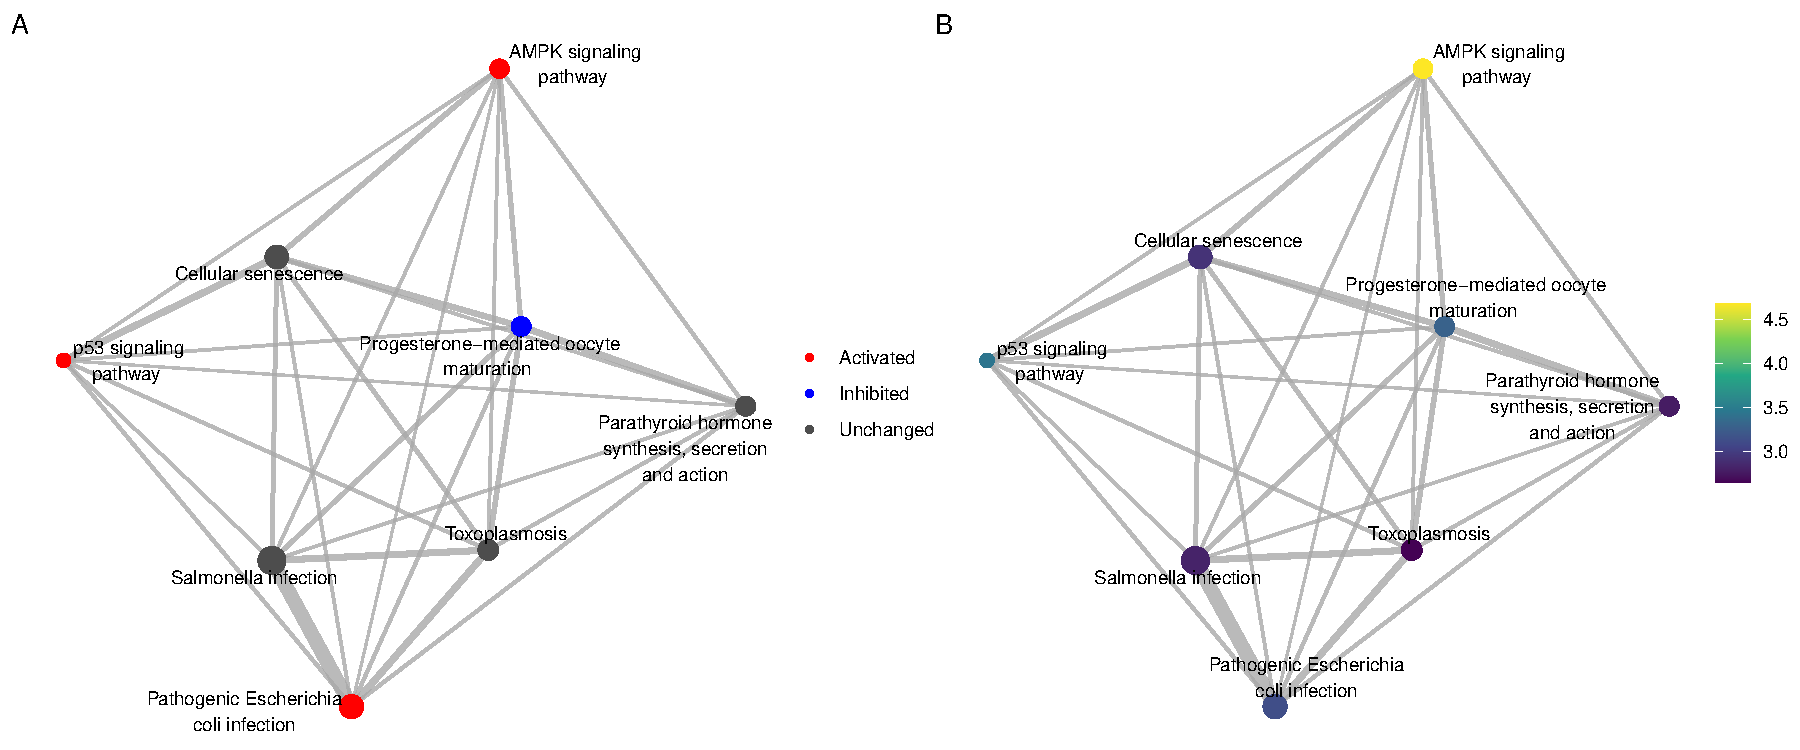
\includegraphics[width=1\linewidth]{sSNAPPY_paper_files/figure-latex/Figure1-1} 

}

\caption{Significantly perturbed KEGG pathways identified among post-chemotherapy samples using sSNAPPY, colored by (A) pathways’ predicted directions of changes and (B) pathways’ -log10(p-values). Pathways with a FDR < 0.05 in the moderated t-test were included.}\label{fig:Figure1}
\end{figure}

By examining the network structure, we can see that many of the highly connected pathways playing a central role in the network are immune-related. To confirm it and further condense the information, we can summarise the network structures into key biological groups by performing community detection. Widely used in network analysis, community detection is a technique used to identify groups of nodes that are more densely connected than to any other nodes in the network\citep{Newman2004}. sSNAPPY's \texttt{plot\_community()} function is a one-stop shop for applying a community detection algorithm of the user's choice to the network structure and annotating identified communities by the most common pathway category, denoting the main biological processes perturbed in that community. Retrieved directly from the \href{https://www.genome.jp/kegg/pathway.html}{KEGG website}, we have curated the most recent categorisations of KEGG pathways and included it as part of the sSNAPPY package. Annotation of KEGG pathway communities will be automatically completed by calling the in-built database, while analyses involving other pathway databases require user-provided pathway categorisations.

The defaulted Louvain method was applied to the network of significantly perturbed biological pathways and revealed two community structures, where one was annotated to be endocrine system related and the other one was infectious disease-related (Figure \ref{fig:Figure2}).

\begin{Shaded}
\begin{Highlighting}[]
\NormalTok{sSNAPPY}\SpecialCharTok{::}\FunctionTok{plot\_community}\NormalTok{(}
    \AttributeTok{normalisedScores =}\NormalTok{ sigPathway, }
        \AttributeTok{gsTopology =}\NormalTok{ gsTopology, }
        \AttributeTok{colorBy =} \StringTok{"robustZ"}\NormalTok{, }
\NormalTok{    ) }\SpecialCharTok{+}
    \FunctionTok{theme}\NormalTok{(}
        \AttributeTok{panel.border =} \FunctionTok{element\_blank}\NormalTok{(), }
        \AttributeTok{panel.background =} \FunctionTok{element\_blank}\NormalTok{()}
\NormalTok{    )}
\end{Highlighting}
\end{Shaded}

\begin{figure}

{\centering 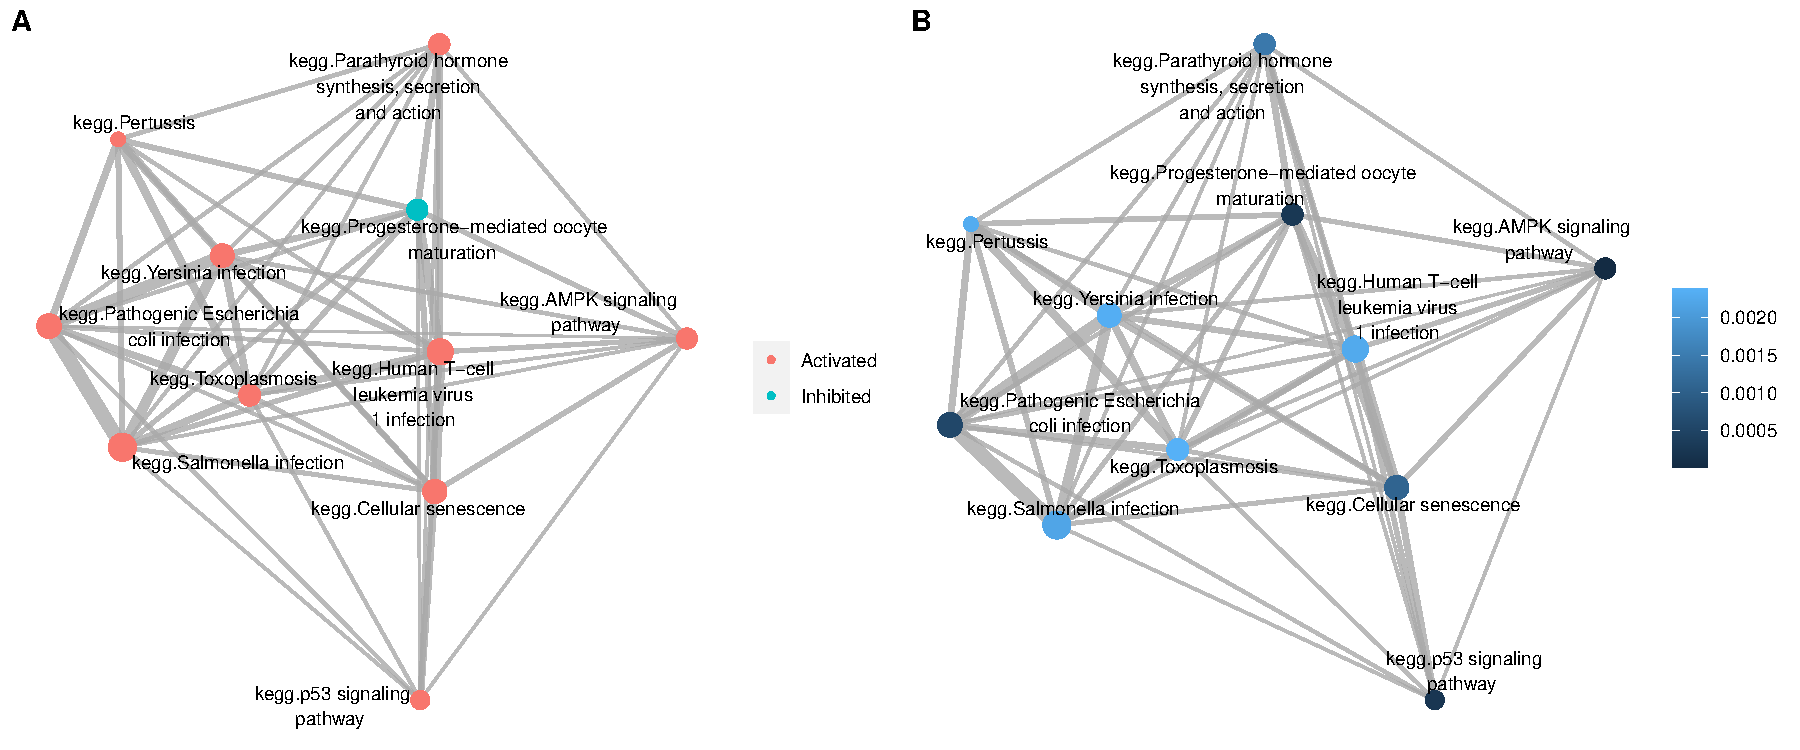
\includegraphics[width=0.8\linewidth]{sSNAPPY_paper_files/figure-latex/Figure2-1} 

}

\caption{Significantly perturbed KEGG pathways identified among post-chemotherapy samples using sSNAPPY, colored by (A) pathways’ predicted directions of changes and (B) pathways’ -log10(p-values). Pathways with a FDR < 0.05 in the moderated t-test were included.}\label{fig:Figure2}
\end{figure}

Inferred directly from the expression matrix, a key advantage of sSNAPPY is that it does not require the prior definition of differentially expressed genes, which is not always detectable in clinical datasets. However, knowing the genes that are implicated in perturbing biological pathways, particularly those that affect multiple gene-sets, can provide valuable insights for biologists seeking to formulate hypotheses about underlying biological mechanisms. Therefore, sSNAPPY presents another visualisation feature called \texttt{plot\_gs2gene}, which enables the inclusion of pathway genes in network structures. Although defaulted to colour all gene nodes in grey, users can provide a vector of logFCs to colour the genes by their changes in expression. As pathways are often made of hundreds of genes, it is recommended not to plot all genes included in perturbed pathways but filter for genes more likely to be playing a significant role, achieved through only providing logFCs of genes to plot. In this example dataset, we chose to only include genes with the top 500 magnitudes of mean logFCs (Figure \ref{fig:Figure3}).

\begin{Shaded}
\begin{Highlighting}[]
\CommentTok{\# Calculate gene{-}wise mean logFCs}
\NormalTok{meanFC }\OtherTok{\textless{}{-}} \FunctionTok{apply}\NormalTok{(weightedFC}\SpecialCharTok{$}\NormalTok{logFC, }\DecValTok{1}\NormalTok{, mean )}
\CommentTok{\# Extract the top 500 meanFCs}
\NormalTok{top500\_FC }\OtherTok{\textless{}{-}}\NormalTok{ meanFC }\SpecialCharTok{\%\textgreater{}\%}
    \FunctionTok{abs}\NormalTok{() }\SpecialCharTok{\%\textgreater{}\%}
    \FunctionTok{sort}\NormalTok{(}\AttributeTok{decreasing =} \ConstantTok{TRUE}\NormalTok{, ) }\SpecialCharTok{\%\textgreater{}\%}
\NormalTok{    .[}\DecValTok{1}\SpecialCharTok{:}\DecValTok{500}\NormalTok{] }
\end{Highlighting}
\end{Shaded}

Since pathway topologies were retrieved in Entrez IDs, by default, genes' Entrez IDs will be used to annotate gene nodes in the plot. However, users can provide a data.frame mapping Entrez IDs to their chosen identifiers through the mapRownameTo parameter. A data.frame converting Entrez IDs to ensemble gene names has been made available as part of the package.

\begin{Shaded}
\begin{Highlighting}[]
\CommentTok{\# Read in built{-}in data.frame entrez2name that matches genes’ }
\CommentTok{\# Entrez IDs to gene names}
\FunctionTok{load}\NormalTok{(}\FunctionTok{system.file}\NormalTok{(}\StringTok{"extdata"}\NormalTok{, }\StringTok{"entrez2name.rda"}\NormalTok{, }\AttributeTok{package =} \StringTok{"sSNAPPY"}\NormalTok{))}
\FunctionTok{head}\NormalTok{(entrez2name)}
\end{Highlighting}
\end{Shaded}

\begin{verbatim}
## # A tibble: 6 x 3
##   gene_id         mapTo   entrezid          
##   <chr>           <chr>   <chr>             
## 1 ENSG00000223972 DDX11L1 ENTREZID:84771    
## 2 ENSG00000223972 DDX11L1 ENTREZID:727856   
## 3 ENSG00000223972 DDX11L1 ENTREZID:100287102
## 4 ENSG00000223972 DDX11L1 ENTREZID:100287596
## 5 ENSG00000223972 DDX11L1 ENTREZID:102725121
## 6 ENSG00000227232 WASH7P  ENTREZID:653635
\end{verbatim}

\begin{Shaded}
\begin{Highlighting}[]
\CommentTok{\# Plot the pathway{-}gene network for genes with top 500 }
\CommentTok{\#magnitudes of mean FCs and label gene nodes by gene names}
\NormalTok{sSNAPPY}\SpecialCharTok{::}\FunctionTok{plot\_gs2gene}\NormalTok{(}
    \AttributeTok{normalisedScores =}\NormalTok{ sigPathway, }
    \AttributeTok{gsTopology =}\NormalTok{ gsTopology, }
    \AttributeTok{colorGS\_By =} \StringTok{"robustZ"}\NormalTok{, }
    \AttributeTok{mapEntrezID =}\NormalTok{ entrez2name, }
    \AttributeTok{geneFC =}\NormalTok{ top500\_FC, }
    \AttributeTok{edgeAlpha =} \FloatTok{0.3}\NormalTok{, }
    \AttributeTok{GsName\_size =} \DecValTok{4}
\NormalTok{) }\SpecialCharTok{+}
    \FunctionTok{theme}\NormalTok{(}
        \AttributeTok{panel.border =} \FunctionTok{element\_blank}\NormalTok{(), }
        \AttributeTok{panel.background =} \FunctionTok{element\_blank}\NormalTok{()}
\NormalTok{)}
\end{Highlighting}
\end{Shaded}

\begin{figure}

{\centering 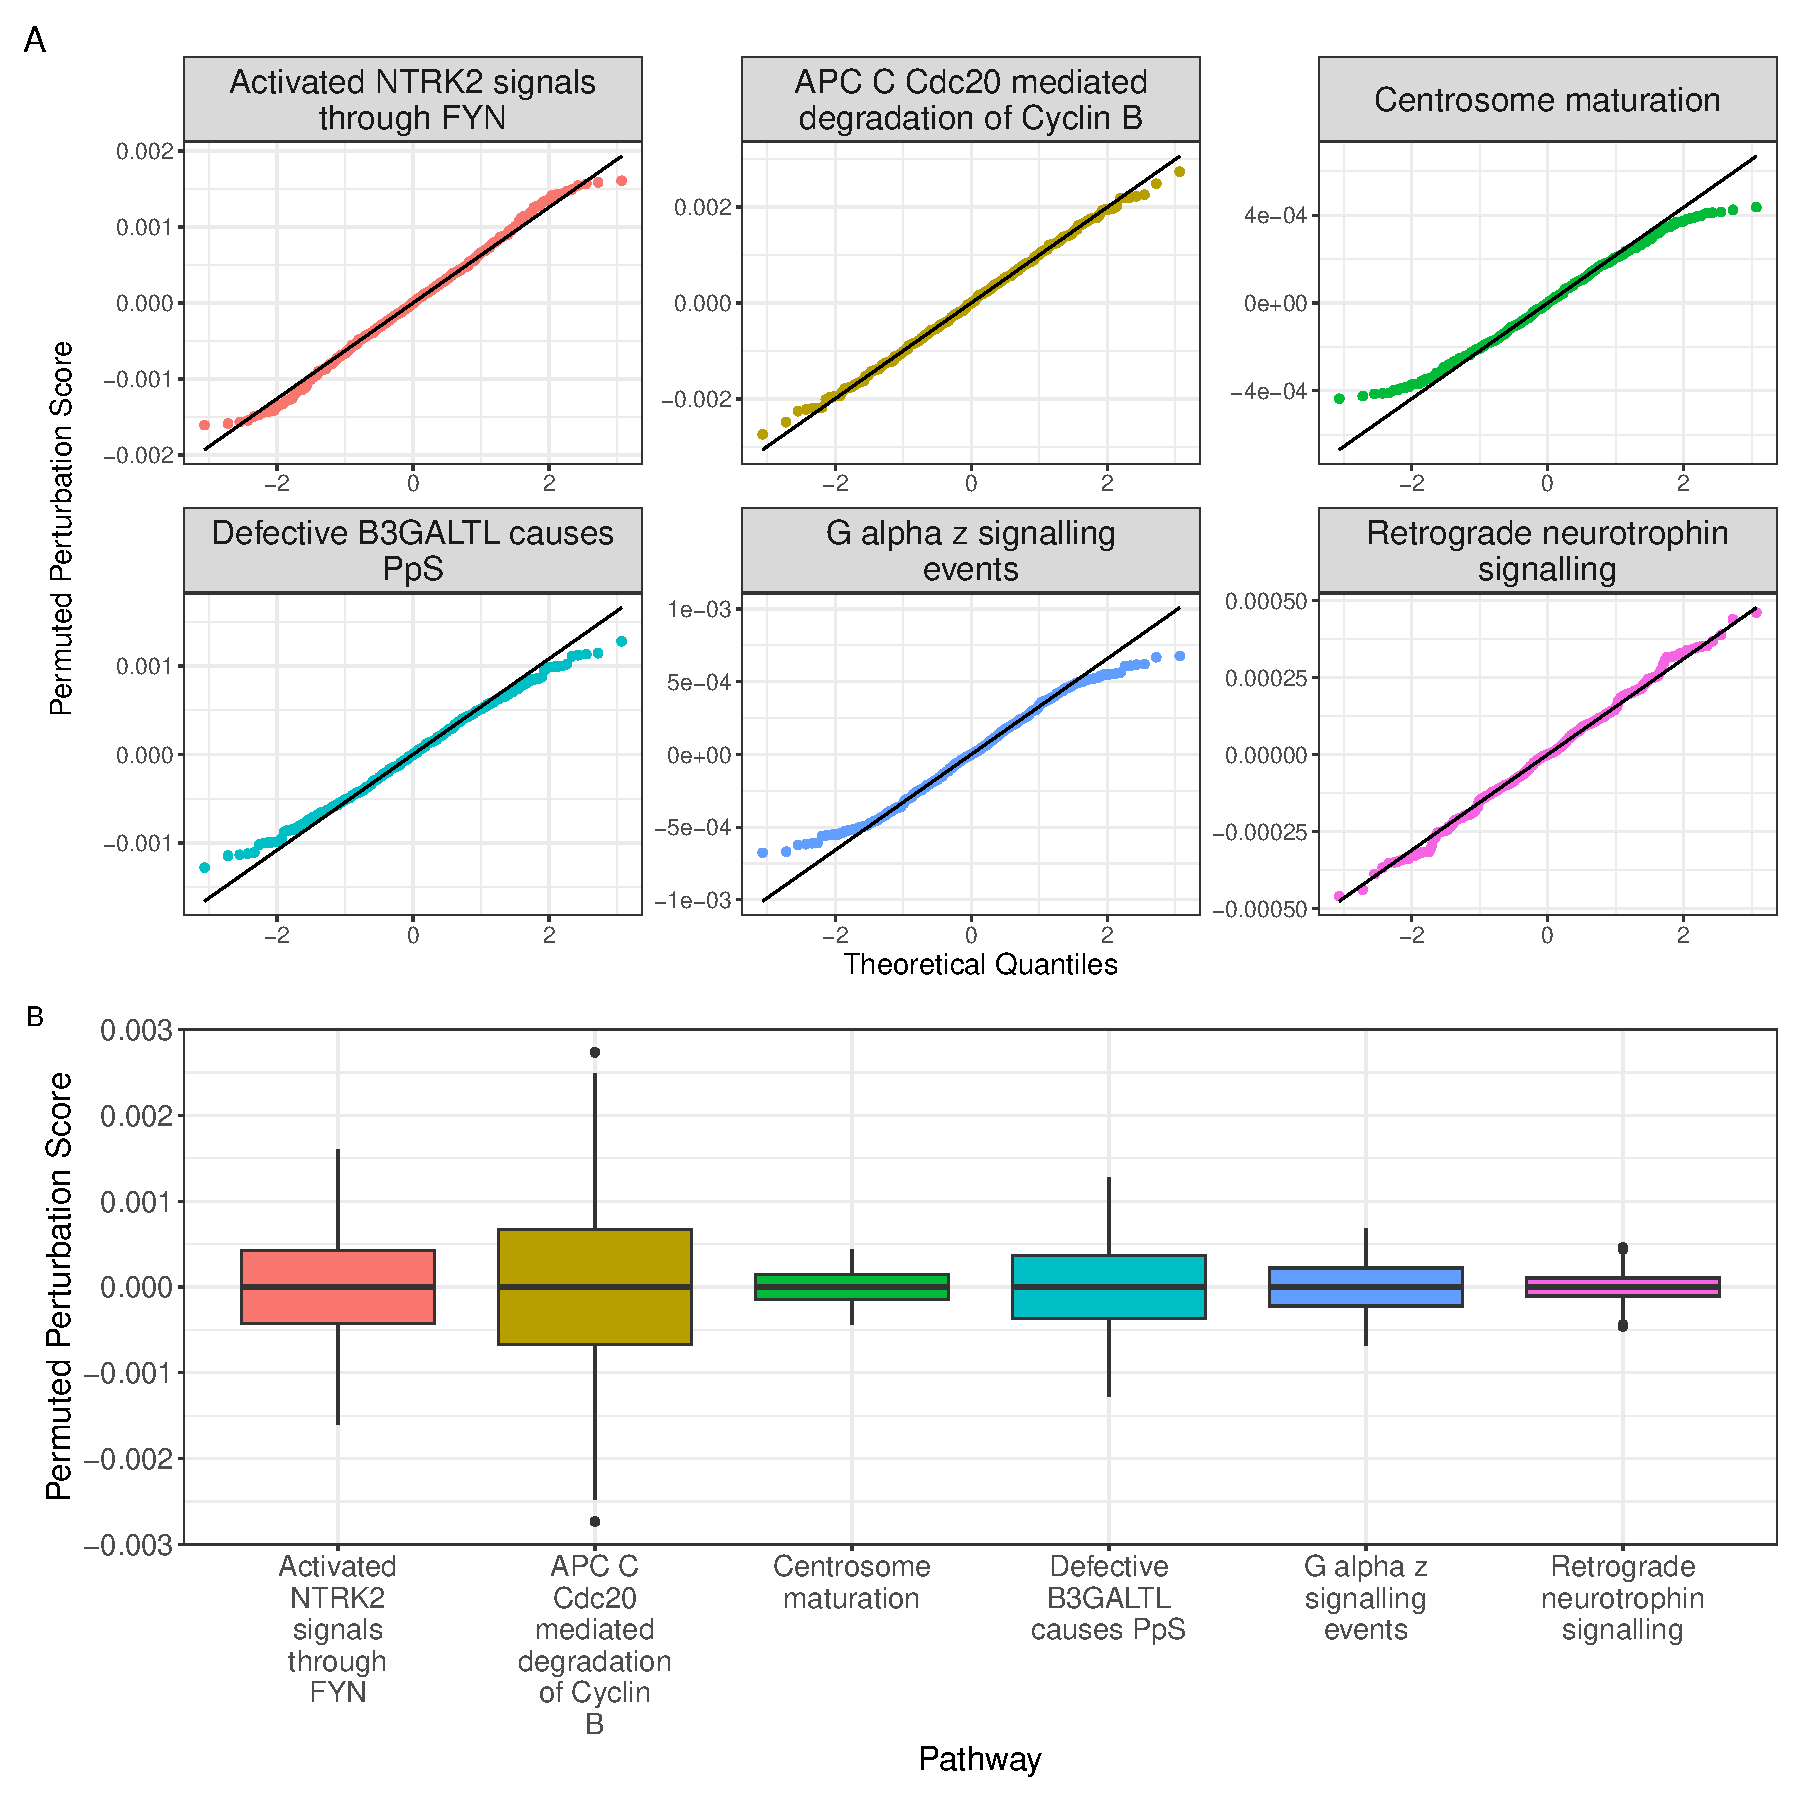
\includegraphics[width=0.8\linewidth]{sSNAPPY_paper_files/figure-latex/Figure3-1} 

}

\caption{Significantly perturbed KEGG pathways identified among post-chemotherapy samples using sSNAPPY, annotated by community structure identified with the Louvain algorithm.2 communities were formed, both of which were annotated by the pathway category that the majority of the pathways belong to. }\label{fig:Figure3}
\end{figure}

\hypertarget{identify-hub-genes-contributing-to-pathway-perturbation}{%
\subsection{Identify hub genes contributing to pathway perturbation}\label{identify-hub-genes-contributing-to-pathway-perturbation}}

If we would like to further investigate a specific pathway and elucidate the key genes that contributed to its perturbation, such as the activation of the ``p53 signalling pathway,'' we can employ a heatmap to display the gene-level perturbation scores of all the genes within the pathway and annotate each column (ie. each sample) by the direction of pathway perturbation in that sample or any other sample metadata using the plot\_gene\_contribution function (Figure \ref{fig:Figure4}).

\begin{Shaded}
\begin{Highlighting}[]
\FunctionTok{plot\_gene\_contribution}\NormalTok{(}
    \AttributeTok{genePertScore =}\NormalTok{ genePertScore, }
    \AttributeTok{gsToPlot =} \StringTok{"p53 signaling pathway"}\NormalTok{, }
    \AttributeTok{metadata =}\NormalTok{ dplyr}\SpecialCharTok{::}\FunctionTok{filter}\NormalTok{(sample\_meta, treatment }\SpecialCharTok{==} \StringTok{"post{-}NACT"}\NormalTok{) }\SpecialCharTok{\%\textgreater{}\%}
\NormalTok{        dplyr}\SpecialCharTok{::}\FunctionTok{select}\NormalTok{(}\AttributeTok{sample =}\NormalTok{ patient\_id, Stage), }
    \AttributeTok{annotation\_attribute =} \FunctionTok{c}\NormalTok{(}\StringTok{"pathwayPertScore"}\NormalTok{, }\StringTok{"Stage"}\NormalTok{), }
    \AttributeTok{pathwayPertScore =}\NormalTok{ ssPertScore, }
    \AttributeTok{mapEntrezID =}\NormalTok{ entrez2name}
\NormalTok{)}
\end{Highlighting}
\end{Shaded}

\begin{figure}

{\centering 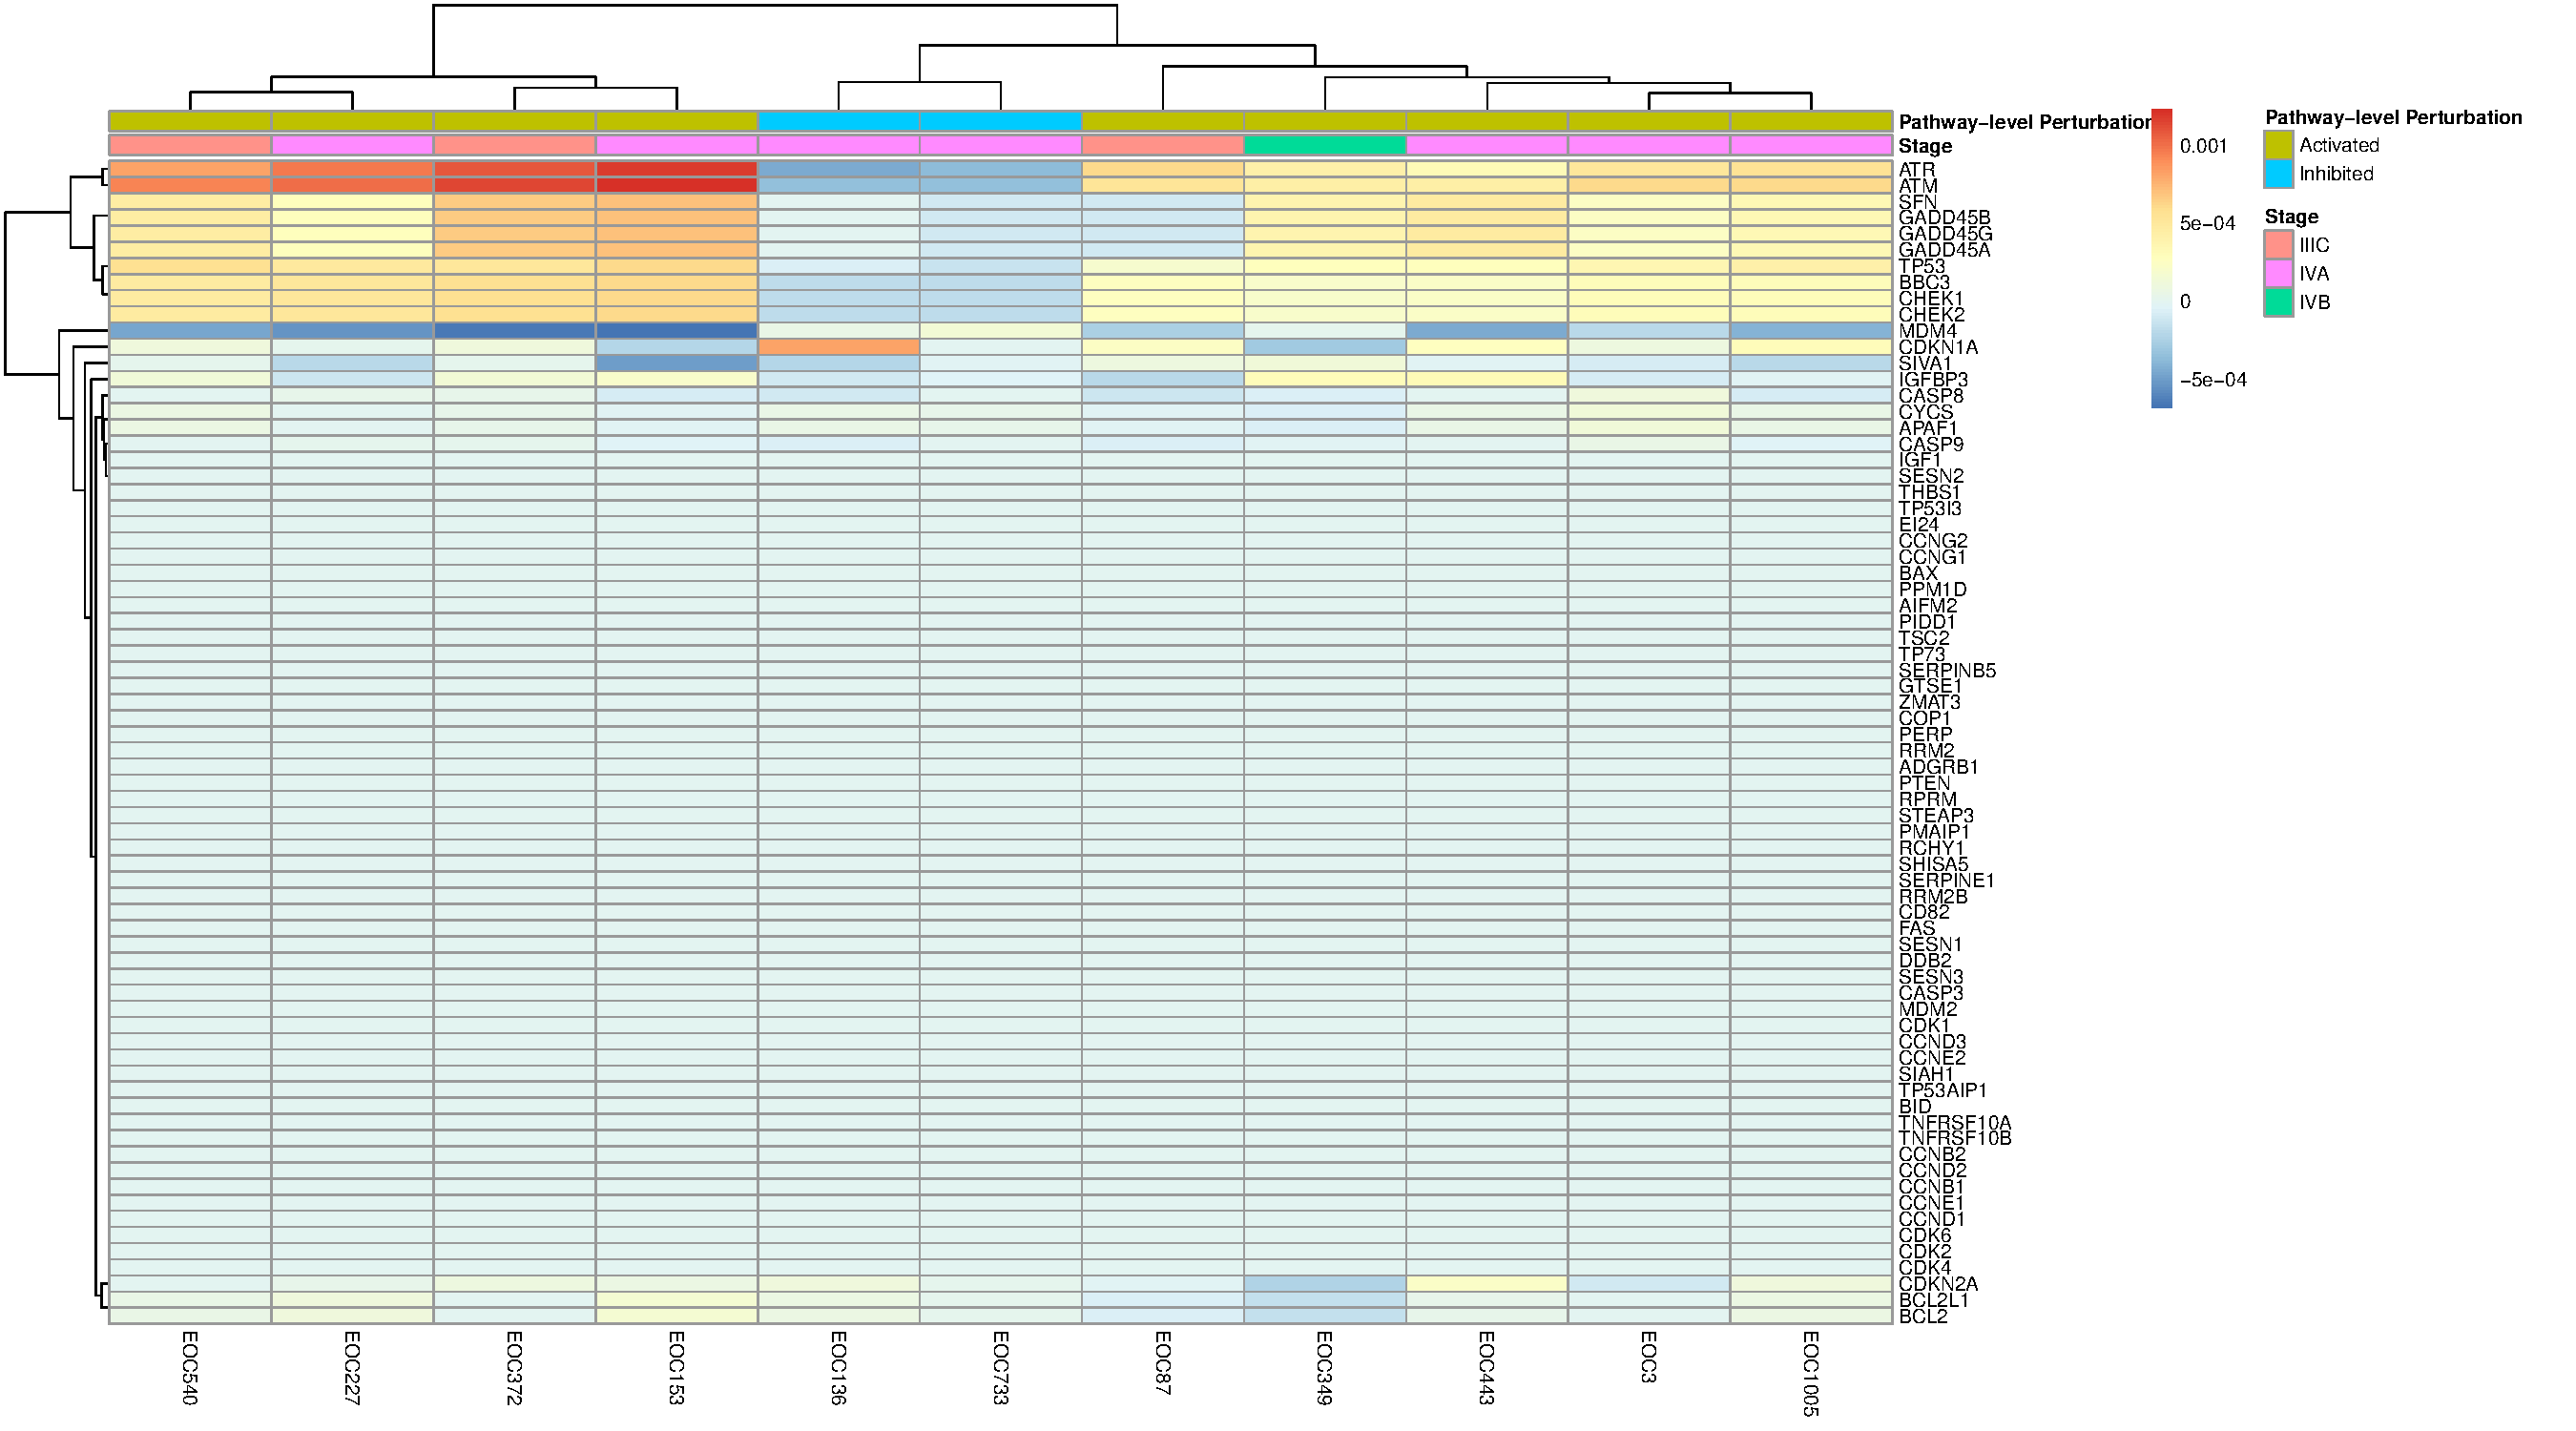
\includegraphics[width=1\linewidth]{sSNAPPY_paper_files/figure-latex/Figure4-1} 

}

\caption{Gene-level perturbation scores of all genes included in the "p53 signalling pathway" pathway in each sample where columns of samples were annotated by pathway-level perturbation and the stages of cancers. Genes ATR and ATM were the key driver of the activation of p53 signalling pathway. }\label{fig:Figure4}
\end{figure}

From this heatmap we can easily identify that the hub genes making the biggest contribution to the activation of p53 signalling pathway upon chemotherapy were gene ART and gene ATM. The Ataxia-telangiectasia mutated (ATM) gene is a well-established oncosuppressor\citep{Moslemi2021}, mutation of which has been observed in many types of cancers\citep{Choi2016}. Also involved in DNA damage repair, the Ataxia telangiectasia and RAD3-related protein kinase (ATR) gene has been shown to be a promising therapeutic target for HGSOC\citep{Li2022}.

\hypertarget{discussion}{%
\section{Discussion}\label{discussion}}

In conclusion, the paper showcased an R/Bioconductor package that offers a novel single-sample pathway perturbation testing approach. sSNAPPY utilizes pathway topology information to compute perturbation scores that predict pathways' potential directions of changes in individual samples. This approach addresses the limitations of current strategies that fail to account for gene-gene interactions encoded by pathway topologies or predict the directionality of pathway activities. By applying sSNAPPY to a public scRNA-seq data collected before and after HGSOC patients were subjected to chemotherapy, we demonstrated its ability to detect significant pathway perturbations of various interesting biological processes beyond what were shown in the original studies. Overall, sSNAPPY presents a promising strategy for single sample-based pathway analysis in RNA-seq data.

\hypertarget{data-availability}{%
\section{Data availability}\label{data-availability}}

The dataset analysed in this manuscript are stored in the data directory of this GitHub repository.

\hypertarget{software-availability}{%
\section{Software availability}\label{software-availability}}

\begin{itemize}
\item
  Software available from: \url{https://bioconductor.org/packages/release/bioc/html/sSNAPPY.html}
\item
  Source code available from: \url{https://github.com/Wenjun-Liu/sSNAPPY}
\item
  Archived source code at time of publication: {[}DOI (found on right hand side of a Zenodo record){]}
\item
  License: \href{https://opensource.org/license/mit/}{MIT}
\end{itemize}

\hypertarget{competing-interests}{%
\section{Competing interests}\label{competing-interests}}

No competing interests were disclosed

\hypertarget{grant-information}{%
\section{Grant information}\label{grant-information}}

Any grants that supported the work must be listed here, including the grant number.

\renewcommand\refname{Acknowledgements}
{\small\bibliography{sample.bib}}

\end{document}
